% =============================================================================
% TCC — Telemetria de uso do kworkflow com OpenTelemetry
% Blockout formal no modelo CCSL/IME-USP (github.com/ccsl-usp/modelo-latex).
% As notas sobre o conteúdo de cada capítulo estão em ../escrita/notas.txt.
% =============================================================================
\documentclass[a4paper,12pt,twoside,english,brazilian]{book}

\usepackage{imegoodies}
\usepackage[thesis]{imelooks}

\graphicspath{{figuras/},{logos/}}

% Bibliotecas TikZ usadas nas figuras (figuras/fig-*.tex)
\usetikzlibrary{arrows.meta, fit, shapes.multipart}

\babeltags{br = brazilian, en = english}

% Capa: "Orientador"/"Coorientador" em vez de "Supervisor"/"Cossupervisor",
% que o modelo usa para TCC (pedido do Octávio, 2026-11-25).
\makeatletter
\addto\captionsbrazilian{%
  \renewcommand\advisorname{Orientador}%
  \renewcommand\coadvisorname[1]{Coorientador}%
}
\makeatother

\addbibresource{bibliografia.bib}

%%%%%%%%%%%%%%%%%%%%%%%%%%%%%%%%%% METADADOS %%%%%%%%%%%%%%%%%%%%%%%%%%%%%%%%%%%

\title{Telemetria de uso do \texttt{kworkflow} com OpenTelemetry}
\translatedtitle{Usage telemetry for \texttt{kworkflow} with OpenTelemetry}

\author{Octávio Gomes Carneiro}

\orientador{Prof. Dr. Paulo Roberto Miranda Meirelles}
\coorientador{David de Barros Tadokoro}

\tipotese{
  tcc,
}

\defesa{
  local={São Paulo},
  data=2026-01-01,
}

\direitos{CC-BY}

%%%%%%%%%%%%%%%%%%%%%%%%%%%%%%%%%%%%%%%%%%%%%%%%%%%%%%%%%%%%%%%%%%%%%%%%%%%%%%%%

\begin{document}

\frontmatter

\pagestyle{plain}

\onehalfspacing

\maketitle

% Reinicia a contagem para que o resumo receba o número "i"
\pagenumbering{roman}

%!TeX root=../main.tex

\palavraschave{}

\keywords{}

\resumo{
}

\abstract{
}


\tableofcontents

%%%%%%%%%%%%%%%%%%%%%%%%%%%%%%%% CAPÍTULOS %%%%%%%%%%%%%%%%%%%%%%%%%%%%%%%%%%%%%

\mainmatter

\pagestyle{mainmatter}

\singlespacing

%!TeX root=../main.tex

\chapter{Introdução}

\label{cap:introducao}

%!TeX root=../main.tex

\chapter{Sobre o kworkflow}

\label{cap:kworkflow}

O kw só se entende a partir do trabalho que ele automatiza, por isso este
capítulo começa pelo desenvolvimento do kernel Linux. Depois apresenta a
ferramenta e termina no dado que o resto do trabalho usa: o registro que o kw
faz do próprio uso e a base local onde ele fica.

\section{O modelo de desenvolvimento do kernel Linux}
\label{sec:modelo-kernel}

O kernel Linux é desenvolvido por milhares de pessoas ao mesmo tempo. Na
versão 7.3, lançada em outubro de 2026, 3.021 desenvolvedores contribuíram
com mais de 18 mil \textit{commits}, que acrescentaram cerca de 650 mil linhas
líquidas ao código; 807 dessas pessoas nunca haviam contribuído antes
\citep{corbet2026stats73}. Nenhuma pessoa consegue revisar esse volume
sozinha, e por isso o projeto é dividido em subsistemas. Cada subsistema
cuida de uma parte do código, como a gerência de memória, a pilha de rede ou
um conjunto de \textit{drivers}, e tem os próprios mantenedores, a própria
árvore \textit{git} e a própria lista de e-mail \citep{kerneldocprocess}. 

Uma alteração sobe por uma cadeia de confiança até a \textit{mainline}, a
árvore mantida por Linus Torvalds e da qual saem as versões oficiais
(Figura~\ref{fig:caminho-patch}). O desenvolvedor envia o trabalho ao
mantenedor do \textit{driver} ou do arquivo que modificou; este o repassa ao
mantenedor do subsistema; e o mantenedor do subsistema, no momento certo do
ciclo, pede a Torvalds que integre a sua árvore à \textit{mainline}, por meio
de um \textit{pull request}\footnote{Aqui, \textit{pull request} é o pedido
para que uma árvore \textit{git} seja integrada a outra, e não o recurso de
mesmo nome do GitHub.}. Torvalds não tem como revisar cada alteração e confia
que os níveis de baixo já fizeram esse trabalho.

\begin{figure}[htbp]
  \centering
  \resizebox{\textwidth}{!}{%!TeX root=../main.tex
% Figura 2.1: caminho de um patch até a mainline.
% Adaptada de Kroah-Hartman (2018), images/kernel_patch_process.svg em
% github.com/gregkh/kernel-development, CC BY-SA 4.0. Mantém a disposição e
% as arestas do original; acrescenta a faixa da interface
% contribuidor-mantenedor e traduz os rótulos.
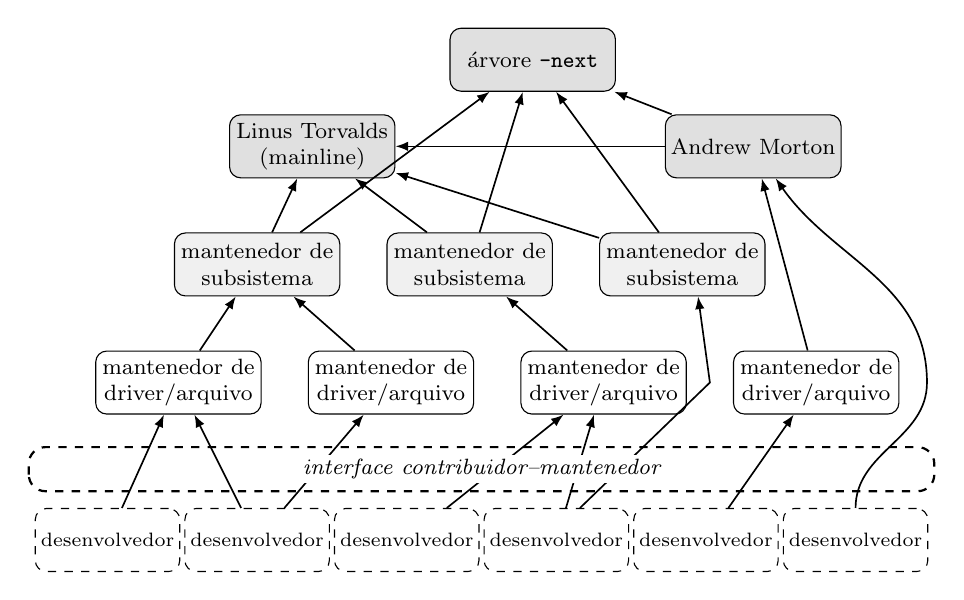
\begin{tikzpicture}[
    x=1cm, y=1cm,
    every node/.style={font=\footnotesize, align=center},
    no/.style={draw, rounded corners=4pt, minimum width=2.1cm,
               minimum height=0.8cm, inner sep=2pt},
    topo/.style={no, fill=black!12},
    subs/.style={no, fill=black!6},
    mant/.style={no, fill=white},
    dev/.style={no, fill=white, minimum width=1.6cm, dashed, font=\scriptsize},
    seta/.style={-{Latex[length=1.6mm]}, semithick},
  ]
  % Topo
  \node[topo] (next)   at (5.4, 6.1) {árvore \texttt{-next}};
  \node[topo] (linus)  at (2.6, 5.0) {Linus Torvalds\\(mainline)};
  \node[topo] (morton) at (8.2, 5.0) {Andrew Morton};

  % Mantenedores de subsistema
  \node[subs] (s1) at (1.9, 3.5) {mantenedor de\\subsistema};
  \node[subs] (s2) at (4.6, 3.5) {mantenedor de\\subsistema};
  \node[subs] (s3) at (7.3, 3.5) {mantenedor de\\subsistema};

  % Mantenedores de driver ou arquivo
  \node[mant] (m1) at (0.9, 2.0) {mantenedor de\\driver/arquivo};
  \node[mant] (m2) at (3.6, 2.0) {mantenedor de\\driver/arquivo};
  \node[mant] (m3) at (6.3, 2.0) {mantenedor de\\driver/arquivo};
  \node[mant] (m4) at (9.0, 2.0) {mantenedor de\\driver/arquivo};

  % Desenvolvedores
  \foreach \i/\x in {1/0.0, 2/1.9, 3/3.8, 4/5.7, 5/7.6, 6/9.5} {
    \node[dev] (d\i) at (\x, 0) {desenvolvedor};
  }

  % Faixa da interface contribuidor-mantenedor (acréscimo desta adaptação)
  \draw[thick, dashed, rounded corners=6pt]
    (-1.0, 0.62) rectangle (10.5, 1.18);

  % Desenvolvedor -> primeiro mantenedor
  \draw[seta] (d1) -- (m1);
  \draw[seta] (d2) -- (m1);
  \draw[seta] (d2) -- (m2);
  \draw[seta] (d4) -- (m3);
  \draw[seta] ([xshift=3mm]d4.north) -- (7.65, 2.0) -- ([xshift=2mm]s3.south);
  \draw[seta] (d3) -- (m3);
  \draw[seta] (d5) -- (m4);
  \draw[seta] (d6.north) to[out=90, in=-90] ([xshift=0.35cm]m4.east) to[out=90, in=-55] (morton);

  % Mantenedor de driver/arquivo -> subsistema
  \draw[seta] (m1) -- (s1);
  \draw[seta] (m2) -- (s1);
  \draw[seta] (m3) -- (s2);
  \draw[seta] (m4) -- (morton);

  % Subsistema -> Linus e -next
  \draw[seta] (s1) -- (linus);
  \draw[seta] (s2) -- (linus);
  \draw[seta] (s3) -- (linus);
  \draw[seta] (s1) -- (next);
  \draw[seta] (s2) -- (next);
  \draw[seta] (s3) -- (next);

  % Andrew Morton -> Linus e -next
  \draw[seta] (morton) -- (linus);
  \draw[seta] (morton) -- (next);
  % Rótulo da faixa por cima das setas
  \node[font=\footnotesize\itshape, fill=white, inner sep=1.5pt]
    at (4.75, 0.9) {interface contribuidor--mantenedor};
\end{tikzpicture}
}
  \caption{Caminho de uma alteração até a \textit{mainline}. Adaptado de
    \citet{kroah2018kerneldev}, sob licença CC BY-SA~4.0; a faixa da
    interface contribuidor--mantenedor foi acrescentada nesta adaptação.}
  \label{fig:caminho-patch}
\end{figure}

A contribuição em si chega por e-mail. A unidade de trabalho é o
\textit{patch}: um arquivo de texto com a diferença entre duas versões do
código e uma mensagem que explica o que mudou e por quê. Parece um
\textit{commit} do \textit{git}, mas formatado para ser enviado a uma lista de
discussão \citep{tadokoro2025sustain}. É na lista que a revisão acontece. Os
mantenedores e outros desenvolvedores respondem ao e-mail com comentários, o
autor corrige e reenvia uma nova versão, e o ciclo se repete até que o
\textit{patch} seja aceito ou abandonado \citep{kerneldocprocess}. Toda essa
troca fica pública e arquivada no
\textit{lore.kernel.org}\footnote{\url{https://lore.kernel.org}}, onde
qualquer pessoa pode ler a discussão de um \textit{patch} do envio ao aceite
\citep{lorekernel, tadokoro2023lore}.

O ritmo das versões é quase fixo: cada ciclo abre com uma janela de cerca de
duas semanas em que os mantenedores enviam a Torvalds o que acumularam, e
segue só com correções até a versão final \citep{kerneldocprocess}. Os
subsistemas aceitam \textit{patches} o tempo todo, mas cada um só chega à
\textit{mainline} no ritmo dos ciclos.

O modelo funciona há mais de trinta anos, mas tem custos. Entre as versões
3.19 (2015) e 6.13 (2025), o código e o número de mantenedores cresceram de
forma constante, enquanto o volume de \textit{commits} por ciclo oscilou sem
tendência de alta \citep{tadokoro2025sustain}. Número de \textit{commits} não
mede esforço, advertem os autores, mas o dado sugere que mais mantenedores não
se traduziram em mais vazão. Parte das contribuições nem chega a ser revisada:
no estudo de \citet{rigby2014peer} sobre as listas do kernel entre 2005 e
2008, 44\% dos \textit{patches} enviados não receberam discussão de revisão. O
problema não diminuiu com o tempo. Ao comentar a chegada recorde de novos
desenvolvedores na versão 7.3, \citet{corbet2026stats73} escreve que os
mantenedores já estão perdendo a capacidade de acompanhar o fluxo. A conclusão
de \citet{corbet2017lfreport} continua valendo: sem as ferramentas certas, um
projeto do tamanho do kernel não conseguiria funcionar sem desabar sob o
próprio peso.

\begin{figure}[htbp]
  \centering
  \resizebox{\textwidth}{!}{%!TeX root=../main.tex
% Figura 2.2: fluxo de desenvolvimento de um patchset.
% Adaptada de Tadokoro, Siqueira e Meirelles (2025), Fig. 1 ("Concept map of
% the patchset development workflow"). Mantém as etapas e os laços de falha;
% traduz os rótulos e destaca as duas etapas que o kw registra (compilação e
% instalação), retomadas na seção 2.4.
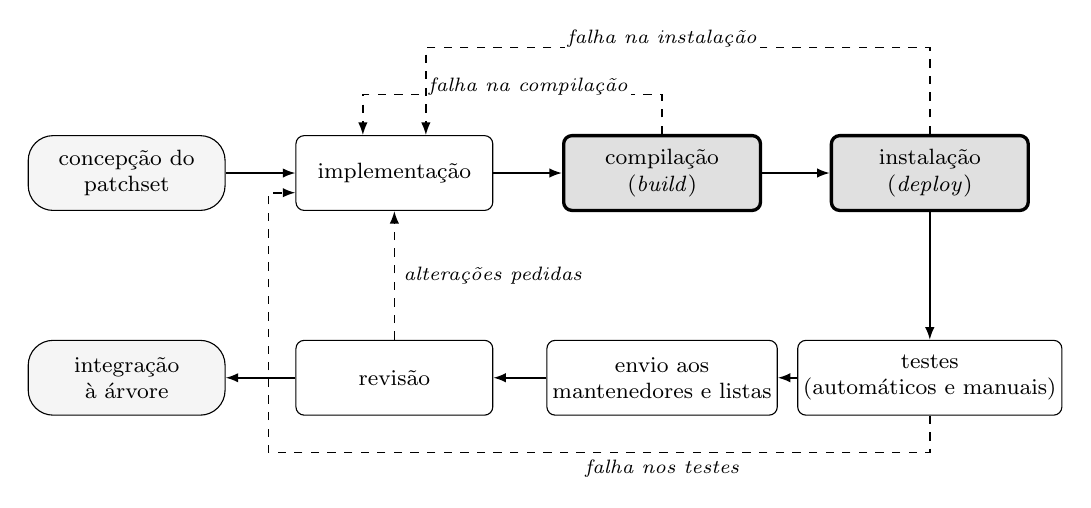
\begin{tikzpicture}[
    x=1cm, y=1cm,
    every node/.style={font=\footnotesize, align=center},
    etapa/.style={draw, rounded corners=3pt, minimum width=2.5cm,
                  minimum height=0.95cm, inner sep=2pt, fill=white},
    reg/.style={etapa, very thick, fill=black!12},
    borda/.style={etapa, rounded corners=9pt, fill=black!4},
    seta/.style={-{Latex[length=1.6mm]}, semithick},
    falha/.style={-{Latex[length=1.6mm]}, semithick, dashed},
    rot/.style={font=\scriptsize\itshape, fill=white, inner sep=1pt},
  ]
  % Linha de cima: da concepção à instalação
  \node[borda] (conc) at (0.0, 2.6) {concepção do\\patchset};
  \node[etapa] (impl) at (3.4, 2.6) {implementação};
  \node[reg]   (comp) at (6.8, 2.6) {compilação\\(\textit{build})};
  \node[reg]   (inst) at (10.2, 2.6) {instalação\\(\textit{deploy})};

  % Linha de baixo: dos testes ao merge
  \node[etapa] (test) at (10.2, 0.0) {testes\\(automáticos e manuais)};
  \node[etapa] (envi) at (6.8, 0.0) {envio aos\\mantenedores e listas};
  \node[etapa] (revi) at (3.4, 0.0) {revisão};
  \node[borda] (merg) at (0.0, 0.0) {integração\\à árvore};

  % Caminho de sucesso
  \draw[seta] (conc) -- (impl);
  \draw[seta] (impl) -- (comp);
  \draw[seta] (comp) -- (inst);
  \draw[seta] (inst) -- (test);
  \draw[seta] (test) -- (envi);
  \draw[seta] (envi) -- (revi);
  \draw[seta] (revi) -- (merg);

  % Laços de falha, todos de volta à implementação
  \draw[falha] (comp.north) -- ++(0, 0.5) -| ([xshift=-4mm]impl.north);
  \node[rot, anchor=south] at (5.1, 3.55) {falha na compilação};
  \draw[falha] (inst.north) -- ++(0, 1.1) -| ([xshift=4mm]impl.north);
  \node[rot, anchor=south] at (6.8, 4.15) {falha na instalação};
  \draw[falha] (test.south) |- (1.8, -0.95) |- ([yshift=-2.5mm]impl.west);
  \node[rot, anchor=north] at (6.8, -1.0) {falha nos testes};
  \draw[falha] (revi.north) -- (impl.south)
    node[rot, midway, right=2pt] {alterações pedidas};
\end{tikzpicture}
}
  \caption{Fluxo de desenvolvimento de um conjunto de \textit{patches}, do
    ponto de vista de quem contribui. As etapas em destaque são as que o
    kworkflow registra, retomadas na Seção~\ref{sec:base-local}. Adaptado de
    \citet{tadokoro2025kw}.}
  \label{fig:fluxo-patchset}
\end{figure}

Uma parte desse custo cai sobre o desenvolvedor antes mesmo de o
\textit{patch} chegar à lista (Figura~\ref{fig:fluxo-patchset}). Ele precisa
compilar o kernel, instalá-lo numa máquina de teste, verificar se a máquina
inicializa e se os testes passam, e só então preparar e enviar o
\textit{patch}. Cada falha o leva de volta à implementação. Nenhuma dessas
etapas é trivial no kernel: uma compilação completa pode levar de minutos a
horas, e a máquina de teste pode ser virtual, remota ou o próprio computador
do desenvolvedor \citep{tadokoro2025kw}. Para cada etapa existe uma
ferramenta: o \texttt{make}, os \textit{scripts} \texttt{checkpatch.pl} e
\texttt{get\_maintainer.pl} que acompanham o código-fonte, o \texttt{git
send-email}, o QEMU. Elas resolvem cada uma a sua parte, e juntá-las num fluxo
de trabalho fica a cargo de cada desenvolvedor, em geral com \textit{scripts}
pessoais que ninguém mais usa \citep{tadokoro2025kw}. O kworkflow nasceu para
reunir esse trabalho num lugar só.

\section{O que é e a que se propõe}
\label{sec:kw-o-que-e}

O kworkflow (kw) é uma ferramenta de software livre, distribuída sob a GPL
versão~2 e escrita em Bash, que reúne numa só interface de linha de comando as
tarefas descritas na seção anterior. O projeto resume o propósito numa frase:
reduzir o custo de preparação do ambiente para quem trabalha com o kernel
Linux e oferecer ferramentas para as tarefas do dia a dia
\citep{kworkflowrepo}. \citet{tadokoro2025kw} o classificam como um
\textit{Developer Automation Workflow System} (DAWS), termo que
\citet{tadokoro2023lore} propôs com a comunidade do projeto por analogia a
\textit{Version Control System}: assim como um sistema de controle de versão
cuida do histórico do código, um DAWS cuida do fluxo de trabalho em volta
dele.

Todos os comandos seguem a forma \texttt{kw <comando> <opções>}, e o projeto
tem hoje duas dezenas deles \citep{tadokoro2025kw}. Eles se dividem em dois
grupos \citep{tadokoro2023lore}. Os comandos práticos agem diretamente sobre o
kernel, como \texttt{kw build}, que compila, e \texttt{kw deploy}, que instala
o kernel compilado numa máquina de teste. Os comandos indiretos não mexem no
kernel, mas melhoram o trabalho em volta dele: gerenciar máquinas remotas,
enviar \textit{patches}, consultar o arquivo das listas, cronometrar sessões
de trabalho. A Tabela~\ref{tab:comandos-kw} reúne alguns comandos de cada
grupo. Para ter uma ideia do que o kw economiza, compilar o
kernel para um processador ARM a partir de um computador x86, com todos os
núcleos e uma \textit{flag} de compilação, exige uma linha de \texttt{make}
com quatro parâmetros; depois de configurado uma vez, o kw reduz isso a
\texttt{kw build} \citep{tadokoro2025kw}.

\begin{table}[htbp]
  \centering
  \caption{Alguns comandos do kworkflow. Seleção a partir da lista completa de
    \citet{tadokoro2025kw}.}
  \label{tab:comandos-kw}
  \begin{tabular}{@{}lll@{}}
    \toprule
    Comando & Tipo & O que faz \\
    \midrule
    \texttt{build}                 & prático  & compila o kernel e os módulos \\
    \texttt{deploy}                & prático  & instala o kernel numa máquina de teste \\
    \texttt{kernel-config-manager} & prático  & gerencia arquivos \texttt{.config} \\
    \texttt{send-patch}            & indireto & envia \textit{patches} por e-mail \\
    \texttt{patch-hub}             & indireto & navega pelos \textit{patches} do \textit{lore.kernel.org} \\
    \texttt{pomodoro}              & indireto & cronometra sessões de trabalho \\
    \texttt{report}                & indireto & mostra estatísticas de uso \\
    \bottomrule
  \end{tabular}
\end{table}


Por dentro, o kw é organizado como um \textit{hub}
(Figura~\ref{fig:arquitetura-kw}). Um único ponto de entrada, o arquivo
\texttt{kw} na raiz do repositório, recebe o comando e o despacha para o
componente correspondente, como \texttt{src/build.sh} para \texttt{kw build}.
Os componentes compartilham bibliotecas em \texttt{src/lib}, que tratam de
tarefas comuns como manipular texto, acessar máquinas remotas ou ler e gravar
no banco de dados. O código que depende de uma distribuição, de uma
arquitetura ou de um subsistema específico, e que por isso muda com
frequência, fica isolado em \textit{plugins} \citep{tadokoro2025kw,
neto2022kw}. A mesma ideia de \textit{hub} vale para a relação com outras
ferramentas: o kw prefere incorporar o que a comunidade já usa, como o
\texttt{git}, o \texttt{checkpatch.pl} e o QEMU, e só escreve uma solução
própria quando nada resolve o problema \citep{tadokoro2025kw}. Isso evita mais
uma camada de \textit{scripts} duplicados, que é justamente o problema
descrito na Seção~\ref{sec:modelo-kernel}.

\begin{figure}[htbp]
  \centering
  \resizebox{0.85\textwidth}{!}{%!TeX root=../main.tex
% Figura 2.3: arquitetura conceitual do kworkflow.
% Adaptada de Tadokoro, Siqueira e Meirelles (2025), Fig. 6 ("kw conceptual
% architecture"). Mantém as camadas do original e destaca as duas
% bibliotecas que gravam os dados de uso (kwlib, onde fica statistics_manager,
% e kw_db), retomadas na
% seção 2.4. Como no original, as ligações são ilustrativas.
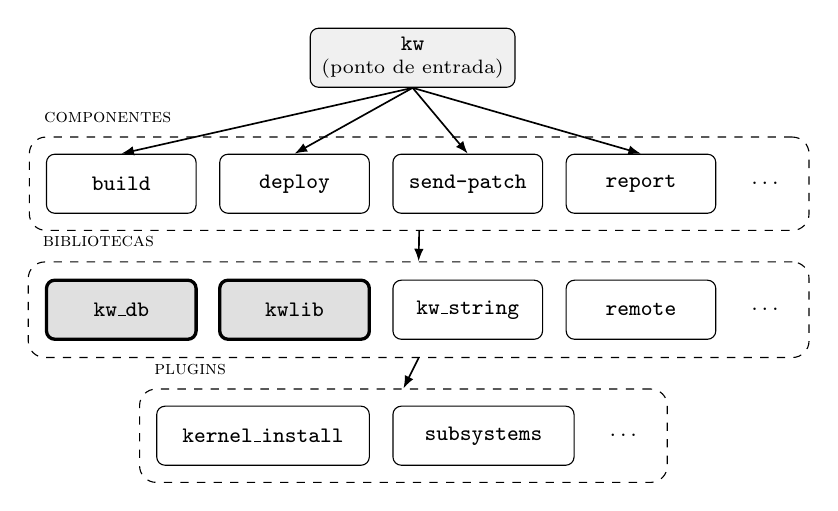
\begin{tikzpicture}[
    x=1cm, y=1cm,
    every node/.style={font=\footnotesize, align=center},
    peca/.style={draw, rounded corners=3pt, minimum width=1.9cm,
                 minimum height=0.75cm, inner sep=2pt, fill=white,
                 font=\footnotesize\ttfamily},
    dado/.style={peca, very thick, fill=black!12},
    camada/.style={draw, dashed, rounded corners=6pt, inner sep=6pt},
    rotulo/.style={font=\scriptsize\scshape, anchor=west},
    seta/.style={-{Latex[length=1.6mm]}, semithick},
  ]
  % Hub
  \node[peca, minimum width=2.6cm, fill=black!6] (hub) at (4.5, 3.6)
    {kw\\[-1pt]{\normalfont\scriptsize(ponto de entrada)}};

  % Componentes
  \node[peca] (c1) at (0.8, 2.0) {build};
  \node[peca] (c2) at (3.0, 2.0) {deploy};
  \node[peca] (c3) at (5.2, 2.0) {send-patch};
  \node[peca] (c4) at (7.4, 2.0) {report};
  \node (c5) at (9.0, 2.0) {\dots};

  % Bibliotecas
  \node[dado] (l1) at (0.8, 0.4) {kw\_db};
  \node[dado] (l2) at (3.0, 0.4) {kwlib};
  \node[peca] (l3) at (5.2, 0.4) {kw\_string};
  \node[peca] (l4) at (7.4, 0.4) {remote};
  \node (l5) at (9.0, 0.4) {\dots};

  % Plugins
  \node[peca, minimum width=2.7cm] (p1) at (2.6, -1.2) {kernel\_install};
  \node[peca, minimum width=2.3cm] (p2) at (5.4, -1.2) {subsystems};
  \node (p3) at (7.2, -1.2) {\dots};

  % Molduras das camadas
  \node[camada, fit=(c1)(c5)] (fc) {};
  \node[camada, fit=(l1)(l5)] (fl) {};
  \node[camada, fit=(p1)(p3)] (fp) {};
  \node[rotulo] at ([xshift=2pt, yshift=7pt]fc.north west) {componentes};
  \node[rotulo] at ([xshift=2pt, yshift=7pt]fl.north west) {bibliotecas};
  \node[rotulo] at ([xshift=2pt, yshift=7pt]fp.north west) {plugins};

  % O hub despacha para os componentes
  \foreach \c in {c1, c2, c3, c4} {
    \draw[seta] (hub.south) -- (\c.north);
  }
  % Os componentes usam bibliotecas e plugins (ligações ilustrativas)
  \draw[seta] (fc.south) -- (fl.north);
  \draw[seta] (fl.south) -- (fp.north);
\end{tikzpicture}
}
  \caption{Arquitetura conceitual do kworkflow. As bibliotecas em destaque
    são as que gravam os dados de uso, descritas na Seção~\ref{sec:base-local}.
    As ligações entre camadas são ilustrativas. Adaptado de
    \citet{tadokoro2025kw}.}
  \label{fig:arquitetura-kw}
\end{figure}

O projeto começou em maio de 2017, como um conjunto de \textit{scripts} para
compilar e instalar o kernel, e com o tempo se tornou uma ferramenta que cobre
o fluxo inteiro \citep{kworkflowrepo, neto2022kw}. O desenvolvimento acontece
no GitHub: as contribuições entram por \textit{pull request} na
\textit{branch} \texttt{unstable}, e a \textit{branch} \texttt{master} recebe
as versões estáveis \citep{neto2022kw}. Rodrigo Siqueira e Matheus Tavares
são os autores principais \citep{tadokoro2025kw}, e boa parte da evolução
recente veio de trabalhos de conclusão de curso do IME-USP.
\citet{neto2022kw} reorganizou a documentação, criou o primeiro modelo de
banco de dados e o comando de envio de \textit{patches};
\citet{tadokoro2023lore} concluiu a migração para o banco e criou o
\texttt{patch-hub}, que integra o kw ao \textit{lore.kernel.org}; e
\citet{souza2025kw} criou o acompanhamento dos \textit{patches} já enviados.
Cada um acrescentou ao kw uma funcionalidade nova. Este trabalho segue a mesma
linha. Propõe uma forma de levar para fora da máquina do desenvolvedor os dados
que o kw já guarda.

Esses dados não são acidentais. Os autores do kw apresentam a ferramenta
também como plataforma de pesquisa: segundo \citet{tadokoro2025kw}, a
infraestrutura de coleta de dados que o kw já tem o torna um bom ponto de
partida para estudar empiricamente o modelo de desenvolvimento do kernel. As
duas seções seguintes descrevem o que, onde e como o kw registra o uso hoje.

\section{O registro de uso e o kw report}
\label{sec:funcionalidades}

O kw registra o próprio uso sem que o usuário precise fazer nada. Ao fim de
cada compilação e de cada instalação, o componente correspondente chama uma
única função, \texttt{statistics\_manager}, com o nome da operação, o momento
em que ela começou, quanto tempo durou e se deu certo
(Programa~\ref{prog:registro}). Hoje só \texttt{build.sh} e
\texttt{deploy.sh} fazem essa chamada, com cinco rótulos: \texttt{build},
\texttt{deploy}, \texttt{modules\_deploy}, \texttt{list} e
\texttt{uninstall}. O banco já prevê rótulos para todos os outros comandos,
mas nenhum deles grava registro. Cada execução termina num de quatro
estados: \texttt{success}, \texttt{failure}, \texttt{interrupted} ou
\texttt{unknown}. A coleta vem ligada por padrão e pode ser desligada pela
opção \texttt{disable\_statistics\_data\_track} do arquivo de configuração
\citep{kworkflowrepo, tadokoro2025kw}. Nada disso sai da máquina.

\begin{program}[htbp]
  \centering
\begin{lstlisting}[language=bash, style=wider]
# src/build.sh, ao fim de kw build
statistics_manager 'build' "$start" "$runtime" 'failure' "$flag"  # falhou
statistics_manager 'build' "$start" "$runtime" '' "$flag"         # sucesso

# src/lib/kwlib.sh
function statistics_manager()
{
  local label_name="$1"
  local start_datetime_in_secs="$2"
  local elapsed_time_in_secs="$3"
  local status=${4:-'success'}
  ...
\end{lstlisting}
  \caption{Registro de uma compilação: as chamadas em \texttt{src/build.sh}
    e o início da função \texttt{statistics\_manager}, em
    \texttt{src/lib/kwlib.sh} \citep{kworkflowrepo}.}
  \label{prog:registro}
\end{program}

O único lugar onde esses registros são lidos é o \texttt{kw report}. Ele
agrega as execuções por dia, semana, mês ou ano e mostra, para cada
operação, quantas vezes ela rodou e o maior, o menor e o tempo médio de
execução (Programa~\ref{prog:report}). A coluna \enquote{Total} é o número de
execuções. O relatório não separa sucessos de
falhas: o estado fica guardado, mas uma compilação que falhou entra na mesma
contagem de uma que deu certo. O mesmo comando resume ainda as sessões do
cronômetro de foco do kw, que ficam fora do escopo deste trabalho. O
\texttt{kw report} roda na máquina de quem gerou os dados e mostra o
resultado só para essa pessoa.

\begin{program}[htbp]
  \centering
\begin{lstlisting}[style=wider, language={}, style=nocolor, numbers=none]
$ kw report --statistics --month
# Statistics Report: month 2026/10
               Total  Max      Min      Average
Build             21 00:23:25 00:03:07 00:12:18
Deploy            15 00:01:10 00:00:28 00:00:45
Modules_deploy     4 00:00:27 00:00:18 00:00:21
List               5 00:00:03 00:00:02 00:00:02
Uninstall          2 00:00:05 00:00:04 00:00:04
\end{lstlisting}
  \caption{Exemplo de saída do \texttt{kw report}. O formato é o do kw; os
    valores são ilustrativos.}
  \label{prog:report}
\end{program}

\section{A base local de estatísticas}
\label{sec:base-local}

Todos esses registros ficam num único arquivo SQLite, o \texttt{kw.db}, no
diretório de dados do usuário. O kw o acessa pela linha de comando do
\texttt{sqlite3}, sem precisar de outra linguagem além do Bash, e esse foi o
critério que levou \citet{neto2022kw} a escolher o SQLite quando o banco foi
criado.

O esquema trata cada uso do kw como um evento ocorrido numa data e
hora \citep{neto2022kw}. A tabela \texttt{event} guarda essa data e hora, e a
tabela \texttt{executed} a estende, com a mesma chave, para dizer qual
operação rodou, quanto tempo levou e em que estado terminou; os nomes das
operações e dos estados ficam em tabelas próprias
(Figura~\ref{fig:esquema-kw}). A mesma tabela \texttt{event} serve de base
para as sessões do cronômetro de foco, que não entram aqui. O código do kw
não escreve nessas tabelas diretamente. A função \texttt{statistics\_manager}
insere uma linha plana na \textit{view} \texttt{statistics\_report}, e um
gatilho \texttt{INSTEAD OF INSERT} distribui o dado entre as tabelas
\citep{kworkflowrepo}. A mesma \textit{view} é por onde o \texttt{kw report}
lê, e as suas seis colunas (identificador, operação, estado, data, hora e
duração) são tudo o que se sabe de cada execução.

\begin{figure}[htbp]
  \centering
  \resizebox{\textwidth}{!}{%!TeX root=../main.tex
% Figura 2.4: parte do esquema do banco do kworkflow usada neste trabalho.
% Desenhada a partir de database/kwdb.sql (commit 2d8a04b). Mostra as tabelas
% do registro de execuções e a view statistics_report, que é a porta de
% entrada (gatilho INSTEAD OF INSERT) e de saída (kw report) desses dados.
% As tabelas do cronômetro de foco (timebox, tag) aparecem só pelo nome.
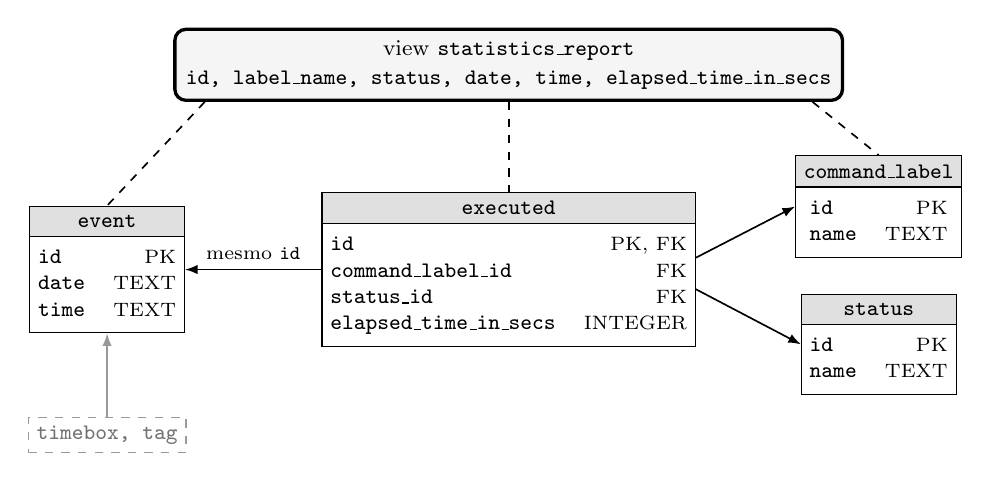
\begin{tikzpicture}[
    x=1cm, y=1cm,
    every node/.style={font=\footnotesize},
    tabela/.style={draw, rectangle split, rectangle split parts=2,
                   rectangle split part fill={black!12, white},
                   inner sep=3pt, font=\footnotesize},
    fora/.style={draw, dashed, text=black!55, draw=black!40,
                 inner sep=3pt, font=\footnotesize\ttfamily},
    visao/.style={draw, very thick, rounded corners=4pt, fill=black!4,
                  inner sep=4pt, align=center, font=\footnotesize},
    fk/.style={-{Latex[length=1.6mm]}, semithick},
    liga/.style={semithick, dashed},
  ]
  % Colunas: nome em \texttt à esquerda, tipo ou chave à direita
  \providecommand{\kwcolunas}{}\renewcommand{\kwcolunas}[1]{%
    \begin{tabular}{@{}l@{\hspace{1.2em}}r@{}}#1\end{tabular}}
  \providecommand{\kwcol}{}\renewcommand{\kwcol}[2]{\texttt{#1} & {\scriptsize #2}\\}

  \node[tabela] (event) at (0, 0) {%
    \texttt{event}
    \nodepart{two}
    \kwcolunas{\kwcol{id}{PK}\kwcol{date}{TEXT}\kwcol{time}{TEXT}}};

  \node[tabela] (executed) at (5.1, 0) {%
    \texttt{executed}
    \nodepart{two}
    \kwcolunas{\kwcol{id}{PK, FK}\kwcol{command\_label\_id}{FK}\kwcol{status\_id}{FK}%
             \kwcol{elapsed\_time\_in\_secs}{INTEGER}}};

  \node[tabela] (label) at (9.8, 0.8) {%
    \texttt{command\_label}
    \nodepart{two}
    \kwcolunas{\kwcol{id}{PK}\kwcol{name}{TEXT}}};

  \node[tabela] (status) at (9.8, -0.95) {%
    \texttt{status}
    \nodepart{two}
    \kwcolunas{\kwcol{id}{PK}\kwcol{name}{TEXT}}};

  \node[fora] (timebox) at (0, -2.1) {timebox, tag};

  % Chaves estrangeiras
  \draw[fk] (executed.west) -- node[above, font=\scriptsize] {mesmo \texttt{id}} (event.east);
  \draw[fk] ([yshift=1.5mm]executed.east) -- (label.west);
  \draw[fk] ([yshift=-2.5mm]executed.east) -- (status.west);
  \draw[fk, draw=black!40] (timebox.north) -- (event.south);

  % A view por cima
  \node[visao] (view) at (5.1, 2.6) {%
    view \texttt{statistics\_report}\\[1pt]
    {\ttfamily id, label\_name, status, date, time, elapsed\_time\_in\_secs}};
  \draw[liga] ([xshift=4mm]view.south west) -- (event.north);
  \draw[liga] (view.south) -- (executed.north);
  \draw[liga] ([xshift=-4mm]view.south east) -- (label.north);
\end{tikzpicture}
}
  \caption{Parte do esquema do \texttt{kw.db} que guarda o registro de
    execuções, com a \textit{view} usada para escrever e ler os dados.
    Desenhado a partir de \texttt{database/kwdb.sql} \citep{kworkflowrepo}.}
  \label{fig:esquema-kw}
\end{figure}

O design serve bem ao que foi feito para servir: o esquema é normalizado,
fácil de consultar e tem um único ponto de escrita. Três propriedades dele,
no entanto, só fazem diferença quando os dados precisam sair da máquina, e as
três voltam no Capítulo~\ref{cap:solucao}.

A primeira é que o identificador
de cada evento cresce na ordem de inserção, o que permite saber o que já foi
lido; como a coluna não é declarada com \texttt{AUTOINCREMENT}, o SQLite pode
reaproveitar o identificador de um evento apagado, embora nenhum código do kw
apague eventos hoje. A segunda é que data e hora são guardadas como texto, em
colunas separadas, no horário local e sem fuso. A terceira é que o esquema não
tem número de versão: todas as tabelas são criadas com \texttt{CREATE TABLE IF
NOT EXISTS}, e o campo \texttt{user\_version} do SQLite fica em zero
\citep{kworkflowrepo}. Quando o esquema foi desenhado, em 2021, os dados
nunca deixavam a máquina de quem os gerou, e as três escolhas eram as
óbvias. Elas continuam corretas para o \texttt{kw report}. O que não existe
ainda é um caminho para que esses dados saiam dali.

%!TeX root=../main.tex

\chapter{Motivação e Objetivos}

\label{cap:motivacao}

\section{Dados de uso como fonte para pesquisa empírica}

\section{O kworkflow como objeto de estudo}

\section{A lacuna de coleta}

\section{Objetivos do trabalho}

%!TeX root=../main.tex

\chapter{A escolha do OpenTelemetry}

\label{cap:opentelemetry}

O caminho que falta ao kw tem um componente central, o OpenTelemetry. Este
capítulo explica o que ele é e justifica a escolha, comparando-o com
alternativas e com o que outras ferramentas de linha de comando fizeram, antes
que o Capítulo~\ref{cap:solucao} mostre como ele é usado.

\section{O que é o OpenTelemetry}
\label{sec:otel-o-que-e}

Instrumentar um programa para emitir dados de telemetria costuma amarrar o
código à ferramenta de análise que recebe esses dados, porque o formato e o
protocolo são os dela. O OpenTelemetry existe para desfazer esse laço. É um
arcabouço de observabilidade, com ferramentas para gerar, exportar e coletar
dados de telemetria como \textit{traces}, métricas e \textit{logs}, e se
declara independente de fornecedor e de ferramenta: o mesmo dado pode ir para
ferramentas diferentes \citep{otel_what_is}. O projeto surgiu em 2019 da fusão
de dois projetos anteriores, o OpenTracing e o OpenCensus, e entrou na Cloud
Native Computing Foundation (CNCF) no estágio inicial, o \textit{sandbox}
\citep{cncf_otel_history_2019}. Em maio de 2026 chegou ao nível
\textit{graduated} \citep{cncf_otel_project}, que o processo da fundação
descreve como o ápice da maturidade de um projeto
\citep{cncf_project_lifecycle}.

O resto do capítulo usa quatro conceitos, apresentados na ordem em que o dado
anda:
\begin{itemize}
  \item \emph{Sinais}: os tipos de dado que o projeto define, isto é,
    \textit{traces}, que mostram o que acontece quando uma requisição é feita,
    métricas, que são medições tomadas durante a execução, e \textit{logs},
    registros de eventos com carimbo de tempo e metadados opcionais
    \citep{otel_signals}, cada um com o próprio estado de estabilidade (o
    protocolo é estável para os três, e o sinal de \textit{profiles} segue em
    desenvolvimento) \citep{otlp_spec_1_11_1}.
  \item \emph{OTLP}: o protocolo que leva qualquer sinal de quem o emite a
    quem o recebe, com dois transportes, gRPC e HTTP; no HTTP, o corpo da
    requisição pode ser protobuf binário ou JSON \citep{otlp_spec_1_11_1}.
  \item \emph{Collector}: um programa pronto que recebe dados de telemetria,
    os processa e os envia a um ou mais sistemas de armazenamento ou análise, organizado em
    \textit{pipelines} de \textit{receivers}, que recebem o dado,
    \textit{processors}, opcionais, que o transformam, e \textit{exporters},
    que o mandam para fora do Collector \citep{otel_collector_architecture}.
  \item \emph{SDKs}: bibliotecas que um programa usa para produzir e exportar
    sinais, uma para cada linguagem atendida, como a de Python
    \citep{otel_python_docs}.
\end{itemize}

Protocolo e SDK são componentes separáveis. A especificação do OTLP define o que
trafega na rede: no transporte HTTP, o cliente envia os dados numa requisição
POST \citep{otlp_spec_1_11_1}. Qualquer programa que monte a mensagem e a
envie fala OTLP, com SDK ou sem ele. Assim, a escolha de quem recebe os dados,
o Collector, fica separada da escolha de como enviá-los, e as seções seguintes
tratam de cada uma à parte.

\section{Critérios de escolha}
\label{sec:criterios}

O motivo central da escolha é o Collector. Ele é um receptor pronto, que já
servia ao caso e se monta por configuração, a partir de \textit{receivers},
\textit{processors} e \textit{exporters} que já existem
\citep{otel_collector_architecture}; o receptor de OTLP e o exportador por
HTTP são componentes estáveis para \textit{logs} na versão usada
\citep{otel_collector_v0_121_0}. Sem ele, seria preciso ler a especificação e
escrever o servidor e o tratamento do protocolo. O segundo motivo é o uso
amplo. Plataformas de análise de vários fornecedores recebem OTLP, como o
Sentry, o PostHog, o Datadog e o New Relic \citep{sentry_otlp, posthog_logs,
datadog_otlp_agent, newrelic_otlp}, de modo que o dado coletado não fica preso
à plataforma escolhida hoje. A maturidade é um ponto distinto, atestado pelo
nível \textit{graduated} da CNCF \citep{cncf_otel_project}.

Do OpenTelemetry, o trabalho usa só o OTLP sobre HTTP e um Collector
configurado, sem SDK. Quem envia precisa apenas de uma requisição HTTP com
corpo JSON, que um programa feito só com a biblioteca padrão do Python monta.
Do lado do servidor, o Collector assume o receptor voltado aos clientes e o
limite de memória, por configuração, sem código de servidor. Sobra um backend
próprio, pequeno, que entende uma parte do OTLP: recebe o corpo que o Collector
reenvia, separa os registros e põe à parte os malformados, descarta os
repetidos, grava num banco SQLite e confirma. O Capítulo~\ref{cap:solucao}
mostra como o Collector e o backend foram montados.

Os critérios da Tabela~\ref{tab:criterios}, de C1 a C9, vêm dos requisitos dos
Capítulos~\ref{cap:kworkflow} e~\ref{cap:motivacao} e de requisitos de
engenharia, e foram fixados antes de olhar as alternativas. O
OpenTelemetry, porém, não entrou na comparação como um candidato entre
outros. Ele era a hipótese de partida, por causa do reuso do Collector, e a
comparação serviu para conferir se a hipótese se sustentava contra os
critérios.

\begin{table}[!ht]
  \centering
  \caption{Critérios da escolha: requisitos (C1 a C8) e preferências (C9).}
  \label{tab:criterios}
  \footnotesize
  \begin{tabular}{@{}>{\raggedright\arraybackslash}p{4.6cm}
                    >{\raggedright\arraybackslash}p{9.6cm}@{}}
    \toprule
    Critério & O que exige \\
    \midrule
    \multicolumn{2}{@{}l}{\textit{Requisitos}} \\
    \addlinespace[2pt]
    C1 Consentimento e filtro por campo
      & O dado só sai após o opt-in, e a privacidade se aplica
        campo a campo, no cliente, por configuração, sem mudar código.\\
    \addlinespace[1pt]
    C2 Extensibilidade
      & Uma fonte ou um atributo novo vai do cliente até a consulta sem
        mudança no protocolo, no Collector nem no backend.\\
    \addlinespace[1pt]
    C3 Um registro por evento, com o tempo do evento
      & Cada evento vai como um registro, com atributos chave e valor livres e
        o momento em que ocorreu, com granularidade de semana; a agregação fica com o backend.\\
    \addlinespace[1pt]
    C4 Cliente em Bash e em Python só com a biblioteca padrão
      & Sem processo residente nem dependência instalada à parte; cada passo
        traduzível para \texttt{sqlite3}, \texttt{jq} e \texttt{curl}.\\
    \addlinespace[1pt]
    C5 Linux, aberto, auto-hospedável
      & Roda em Linux, tem código aberto e pode ser hospedado por quem recebe
        os dados, sem conta em serviço de terceiros.\\
    \addlinespace[1pt]
    C6 Custo operacional baixo
      & Uma máquina, configuração em vez de código de servidor, sem banco ou
        fila obrigatórios para começar.\\
    \addlinespace[1pt]
    C7 Garantia de entrega
      & Confirmação só depois da gravação no backend; reenvio sem duplicar.\\
    \addlinespace[1pt]
    C8 Maturidade e estabilidade
      & Sinal e protocolo estáveis na especificação, versão fixada e histórico
        de mudanças incompatíveis conhecido.\\
    \midrule
    \multicolumn{2}{@{}l}{\textit{Preferências}} \\
    \addlinespace[2pt]
    C9 Reuso de um receptor pronto e amplamente usado
      & O lado servidor e o tratamento do protocolo vêm prontos e
        configuráveis, em vez de lidos da especificação e escritos pelo
        projeto, e o componente tem uso amplo.\\
    \bottomrule
  \end{tabular}
\end{table}


\section{Alternativas consideradas}
\label{sec:alternativas}

A comparação põe o OpenTelemetry ao lado de três outras formas de montar o
caminho inteiro, do cliente ao backend: não reusar nada e escrever um
receptor próprio, usar um sistema de métricas, ou usar uma plataforma de
análise pronta. Cada uma representa um grupo; outras opções examinadas
ficaram de fora, e a lista não é exaustiva. Aqui se pergunta por que o
OpenTelemetry. Como ele é usado, com que sinal, que cliente e que
codificação, é escolha do Capítulo~\ref{cap:solucao}. Os critérios estão na
Tabela~\ref{tab:criterios}, e a parte seguinte explica as avaliações de cada
alternativa, resumidas na Tabela~\ref{tab:alternativas}, ao fim da seção. As
ressalvas do próprio OpenTelemetry ficam para a Seção~\ref{sec:limites-otel}.


A primeira alternativa é um \textbf{servidor HTTP próprio}, que recebesse JSON
no formato que o kw quisesse. É o caminho mais curto no começo e, no papel,
atende quase todos os critérios. Tem também vantagens sobre a escolha: a
superfície é menor, sem Collector e sem as regras do JSON do OTLP, e o
contrato de erro é do projeto. Seu custo está no C9: seria preciso escrever o
receptor, a validação e os limites, e manter um formato que nenhuma outra
ferramenta lê; na prática, é o backend próprio deste trabalho sem o Collector
na frente. Pelo mesmo motivo, a operação e as regras de sucesso e de
retentativa (C6 e C7) seriam código do projeto. A maturidade (C8) também é uma
ressalva: um componente escrito e mantido pelo próprio projeto começa sem
histórico que permita julgá-lo maduro, e chegar lá pediria trabalho que vai
além do código, como formar e manter uma comunidade em torno dele. Essa linha
da tabela é avaliação deste trabalho, sem fonte externa.

O Kieker, uma
ferramenta de monitoramento com formato de registro próprio, mostra o que
acontece quando se quer reusar outra ferramenta: para alimentar o ExplorViz,
de visualização, foi preciso transformar os seus registros de fluxo de
controle em \textit{traces} do OpenTelemetry, exportados por gRPC ou Zipkin
\citep{reichelt2024kieker}. Ler essa ponte como um custo do formato próprio é
interpretação deste trabalho, não do artigo.

A segunda alternativa é o \textbf{Prometheus com o Pushgateway}. O Prometheus
coleta métricas puxando-as dos processos monitorados, por HTTP, e a visão
geral do projeto indica um intermediário, o Pushgateway, para trabalhos de
vida curta \citep{prometheus_overview}, e um comando do kw, na leitura deste
trabalho, é desse tipo. A documentação, porém, aponta dois problemas. O
Pushgateway recusa envios que tragam carimbo de tempo, de modo que o momento
do evento se perde (C3) \citep{pushgateway_readme}. Além disso, a documentação
diz que o uso válido do Pushgateway é, em geral, guardar o resultado de um
trabalho em lote de um serviço, e que ele nunca esquece as séries recebidas
\citep{prometheus_pushing}, o que sugere que muitas instalações independentes,
cada uma com seus eventos, não são o caso previsto; e, como cada atributo novo
vira um rótulo novo e cria séries novas, uma fonte nova pesa sobre esse
acúmulo (C2).

No Pushgateway, as métricas ficam agrupadas por uma chave, e um envio por PUT
substitui todas as métricas do grupo \citep{pushgateway_readme}, então o
cliente teria de reenviar o estado do grupo, não só os eventos novos (C4). O
filtro de rótulos fica no Prometheus que coleta, depois que o dado chegou
inteiro ao Pushgateway (C1) \citep{prometheus_config_v3_16_0}. O Pushgateway
não guarda os dados em disco por padrão \citep{pushgateway_readme}, e nada
nele confirma que um envio foi gravado pelo Prometheus que o coleta (C7). São,
por fim, dois serviços a operar (C6).

A terceira alternativa é uma plataforma de análise de produto, o
\textbf{PostHog}, que substituiria o caminho inteiro, do recebimento à
consulta. É código aberto, sob a licença MIT fora do diretório \texttt{ee/}
(C5) \citep{posthog_license}, e aceita eventos por uma API própria e
\textit{logs} por OTLP \citep{posthog_capture, posthog_logs}; escolher OTLP,
portanto, não fecha a porta a uma plataforma como essa. Seu ponto forte é o
que o C9 pede: o armazenamento e a consulta vêm prontos, com mais recursos que
os do backend próprio.

O PostHog também filtra propriedades dos eventos
imediatamente antes de gravá-los \citep{posthog_realtime_transformations}, mas
no servidor, depois do envio. Nas páginas consultadas, nenhuma diz se esse
recurso funciona na instalação própria, e a lista do que se perde ao hospedar
o PostHog por conta própria inclui os \textit{data pipelines}, seção onde ele
está documentado \citep{posthog_selfhost_disclaimer}. A API de captura exige
um identificador da pessoa em cada evento, enquanto o kw usaria só um
identificador aleatório de instalação (C1), e responde 200 mesmo a eventos que
não grava \citep{posthog_capture}; só a versão mais nova da API diz, evento a
evento, o que foi gravado (C7) \citep{posthog_capture_v1}. Contra ele pesa o custo
de operação (C6): a instalação própria pede o equivalente a uma máquina com
4 vCPU e 16~GB de memória \citep{posthog_selfhost}, para uma escala de cerca
de um envio por instalação por dia (Capítulo~\ref{cap:solucao}), e não tem
suporte oficial (C8) \citep{posthog_selfhost}.

\begin{table}[!ht]
  \centering
  \newcommand*{\cA}[1][]{A#1}
  \newcommand*{\cR}[1][]{\cellcolor{black!10}R#1}
  \newcommand*{\cN}[1][]{\cellcolor{black!25}N#1}
  \newcommand*{\cQ}[1][]{\textbf{?}#1}
  \newcommand*{\cNA}[1][]{n/a#1}
  \newcommand*{\nosso}{\textsuperscript{*}}
  \small
  \setlength{\tabcolsep}{3pt}
  \begin{threeparttable}
    \caption{Alternativas consideradas, avaliadas pelos critérios da
      Tabela~\ref{tab:criterios}.}
    \label{tab:alternativas}
    \begin{tabular}{@{}>{\raggedright\arraybackslash}p{3.9cm}
                      *{9}{>{\centering\arraybackslash}p{0.92cm}}@{}}
      \toprule
       & \makecell{C1\\[-2pt]\scriptsize filtro} & \makecell{C2\\[-2pt]\scriptsize extens.}
       & \makecell{C3\\[-2pt]\scriptsize evento} & \makecell{C4\\[-2pt]\scriptsize cliente}
       & \makecell{C5\\[-2pt]\scriptsize aberto} & \makecell{C6\\[-2pt]\scriptsize custo}
       & \makecell{C7\\[-2pt]\scriptsize entrega} & \makecell{C8\\[-2pt]\scriptsize matur.}
       & \makecell{C9\\[-2pt]\scriptsize reuso} \\
      \midrule
      OpenTelemetry (OTLP e Collector), a escolha
        & \cA[\nosso] & \cA[\nosso] & \cA & \cA[\nosso] & \cA
        & \cR & \cR & \cR & \cA \\
      Endpoint HTTP/JSON próprio
        & \cR[\nosso] & \cA[\nosso] & \cA[\nosso] & \cA[\nosso] & \cA[\nosso]
        & \cR[\nosso] & \cR[\nosso] & \cR[\nosso] & \cN[\nosso] \\
      Prometheus com Pushgateway
        & \cR & \cR & \cN & \cR & \cA
        & \cR & \cN & \cA & \cA \\
      PostHog (plataforma de análise)
        & \cR & \cA & \cA & \cA & \cR
        & \cN & \cR & \cR & \cA \\
      \bottomrule
    \end{tabular}
    \begin{tablenotes}
      \footnotesize
      \item A: atende; R: atende com ressalva; N: não atende; *: avaliação
        deste trabalho, sobre o design ou o repositório, sem fonte externa
        (Capítulo~\ref{cap:solucao}).
        Critérios na Tabela~\ref{tab:criterios}.
      \item Justificativas na Seção~\ref{sec:alternativas}.
    \end{tablenotes}
  \end{threeparttable}
\end{table}


\section{Precedentes em ferramentas de linha de comando}
\label{sec:precedentes}

O Capítulo~\ref{cap:motivacao} citou quatro ferramentas que já enfrentaram a
questão do kw: a cadeia de ferramentas do Go, o Debian Popularity Contest
(popcon), o Homebrew e a interface de linha de comando do .NET. Todas rodam
como processos curtos na máquina de quem as usa, sem um serviço próprio sempre
ligado, e precisam levar dados de muitas máquinas para um lugar central. Aqui
interessa como cada uma pede consentimento, envia, guarda o estado do envio e
identifica a máquina, não o que coleta, que não é critério para o kw. A
Tabela~\ref{tab:precedentes}, ao fim da seção, resume as quatro e, na última
linha, como o kw trata cada um desses pontos.

A cadeia de ferramentas do \textbf{Go} guarda contadores na máquina,
agrega-os em relatórios semanais e, por padrão, nunca os envia
\citep{go_telemetry_doc}. O design
publicado por Russ Cox em fevereiro de 2023 era opt-out
\citep{cox_telemetry_design_2023}; dezesseis dias depois, após debate público,
passou a opt-in \citep{coxsw2023optin}, e é assim que a telemetria saiu no
Go 1.23 \citep{go_release_1_23}. Os relatórios enviados, diz o design, não
incluem identificador de nenhum tipo
\citep{cox_telemetry_design_2023}. O relatório vai por POST, em JSON; só
depois de uma resposta 200 sai da fila local, e uma resposta 4xx o descarta
\citep{golang_telemetry}. Na discussão pública do design, Cox disse entender
o OpenTelemetry como organizado em torno de um fluxo de eventos e escreveu
que evitar esse fluxo é uma das formas de reduzir o impacto sobre a
privacidade. Um desenvolvedor do OpenTelemetry concordou, disse que o SDK de
Go poderia ser adaptado, mas que não valia o esforço, e que o OpenTelemetry
poderia ser um bom lugar para uma telemetria assim
\citep{go_discussion_58409}.

O \textbf{popcon} coleta dados de uso para orientar o próprio projeto, e o
artigo do kw já o toma como referência (Seção~\ref{sec:dados-de-uso}). A
participação é opt-in, com \enquote{não} como resposta padrão na instalação.
Cada máquina recebe um identificador aleatório de 128 bits, e um novo envio
sobrescreve o último de mesmo identificador; o servidor publica todo dia um
resumo que junta os envios e não traz os identificadores
\citep{popcon_package_1_78}. O próprio popcon avisa que nenhum envio é
completamente anônimo \citep{popcon_package_1_78}, ponto que o
Capítulo~\ref{cap:privacidade} retoma.

O \textbf{Homebrew} mostra um aviso antes de ativar a coleta, que pode ser
desligada, e a carga não tem identificador de usuário nem campo de endereço IP
\citep{brew_analytics}. O envio é um \texttt{curl} por HTTPS em processo
destacado, com tempo máximo de 3 segundos \citep{brew_analytics_code}, para
não atrasar o comando. As falhas são silenciosas \citep{brew_analytics}, e não
há fila nem estado de envio em disco \citep{brew_analytics_code}.

A \textbf{interface de linha de comando do .NET} é a única das quatro que adota o
OpenTelemetry, e ainda só no ramo principal e em versões de prévia. A troca
entrou em abril de 2026 \citep{dotnet_sdk_pr_53181} e está nas prévias 11.x a
partir da quarta; desde a quinta, o envio por OTLP depende de uma variável de
ambiente \citep{dotnet_sdk_telemetryclient_rc3}. As versões estáveis 10.x
ainda usam o cliente anterior, que guarda os envios numa fila em disco e os
reenvia quando o erro permite \citep{dotnet_sdk_v10_0_404}. A telemetria é
opt-out, ligada por padrão nas distribuições da Microsoft e desligável por
variável de ambiente; o identificador da máquina é o SHA-256 do endereço MAC,
e os agregados são publicados sob licença Creative Commons
\citep{dotnet_cli_telemetry}. É, portanto, um projeto grande da mesma
categoria levando a sua telemetria para o OpenTelemetry, ainda fora das
versões estáveis, e usando o SDK, que na plataforma .NET é nativo.

O \textbf{kw} usa o opt-in, como o Go e o popcon, um identificador aleatório
de instalação, como o popcon, e o envio em segundo plano, sem bloquear o
comando, como o Homebrew. Ele se afasta do Go na forma como os dados são
agregados. No Go, a agregação acontece no cliente, e só o relatório semanal,
já resumido, sai da máquina. No kw, cada evento sai como um registro, e as
agregações são feitas no backend, por consulta, o que deixa qualquer atributo
novo disponível para agrupar sem mudar o cliente (Capítulo~\ref{cap:solucao});
o custo dessa escolha está na Seção~\ref{sec:limites-otel}. Ao contrário do
Homebrew, o kw só marca um registro como enviado depois da confirmação do
backend. Ao contrário do .NET, não envia nada antes do opt-in, não deriva o
identificador de um dado da máquina e, escrito em Bash, não usa SDK.

\begin{table}[!ht]
  \centering
  \footnotesize
  \setlength{\tabcolsep}{4pt}
  \begin{threeparttable}
    \caption{Como quatro ferramentas de linha de comando pedem o
      consentimento, enviam os dados, tratam o envio e identificam a
      máquina, e como o kw trata os mesmos pontos.}
    \label{tab:precedentes}
    \begin{tabular}{@{}>{\raggedright\arraybackslash}p{1.7cm}
                      >{\raggedright\arraybackslash}p{3.0cm}
                      >{\raggedright\arraybackslash}p{3.0cm}
                      >{\raggedright\arraybackslash}p{3.4cm}
                      >{\raggedright\arraybackslash}p{2.9cm}@{}}
      \toprule
      Ferramenta & Consentimento & Como e para onde envia & Estado de envio
        & Identificador \\
      \midrule
      Go
        & Opt-in: o modo padrão, \texttt{local}, guarda os dados e nunca envia
        & Relatório semanal em JSON, por POST, para
          \texttt{telemetry.go.dev}
        & Após a resposta 200, o relatório vai para a pasta
          \texttt{upload/}; um erro 4xx o apaga
        & Nenhum: os relatórios não trazem identificador de nenhum tipo,
          segundo o design de 2023 \\
      \addlinespace
      Debian popcon
        & Opt-in: a resposta padrão na instalação é ``não''
        & POST por HTTP para \texttt{popcon.\allowbreak debian.org}
        & O servidor substitui o envio anterior da mesma máquina pelo novo
        & UUID aleatório de 128 bits por máquina \\
      \addlinespace
      Homebrew
        & Mostra um aviso antes de ativar e pode ser desligada
        & \texttt{curl} em processo destacado, por HTTPS, com tempo máximo de
          3~s
        & Nenhum estado de envio nem fila própria; as falhas são silenciosas
        & Nenhum: o envio não traz identificador de usuário nem campo de
          endereço IP \\
      \addlinespace
      CLI do .NET
        & Ligada por padrão nas distribuições da Microsoft; \mbox{opt-out} por
          variável de ambiente
        & Azure Monitor; nas prévias da versão 11, também OTLP, que depende de
          variável de ambiente a partir da \textit{preview}~5
        & Na versão 10, anterior ao OpenTelemetry: fila em disco e reenvio
          quando o erro permite
        & \textit{Hash} SHA-256 do endereço MAC \\
      \midrule
      kw
        & Opt-in; enquanto não há resposta, o estado é \texttt{ask} e nada é
          enviado; o usuário pode excluir campos do envio
          (\texttt{exclude\_fields}), vazio por padrão
        & Um registro por evento, com o tempo em granularidade de semana, OTLP/HTTP
          com JSON, em segundo plano, sem bloquear o comando, para um
          Collector e daí ao backend
        & Cada evento é marcado como enviado só depois da confirmação do backend
        & UUID aleatório por instalação, criado no opt-in \\
      \bottomrule
    \end{tabular}
    \begin{tablenotes}
      \footnotesize
      \item Justificativas na Seção~\ref{sec:precedentes}. Linha do kw:
        avaliação deste trabalho sobre o repositório
        (Capítulo~\ref{cap:solucao}).
    \end{tablenotes}
  \end{threeparttable}
\end{table}


\section{Limites da escolha}
\label{sec:limites-otel}

Reusar o OpenTelemetry tem um preço, e o primeiro está no Collector, que está
na versão 0.x; e a política de versões do projeto avisa que, nessa faixa, nada
é garantido estável \citep{otel_collector_v0_121_0}. O receptor de OTLP e o
exportador por HTTP, por onde o dado entra e sai, são estáveis para
\textit{logs}; os três \textit{processors} do caminho, o de limite de memória,
o de recurso e o de atributos, estão em beta. As mudanças incompatíveis das
versões 0.119.0 a 0.121.0, esta última a usada, não tocaram nenhum desses
componentes \citep{otel_collector_v0_121_0}. O Collector é também mais um
serviço a operar, ao lado do backend (C6). A versão fica fixada, e cada
atualização precisa ser testada (C8).

O segundo preço está no sinal e no formato. O modelo de dados de \textit{logs}
e o protocolo são estáveis \citep{otel_logs_data_model, otlp_spec_1_11_1}. O
modelo foi declarado estável em março de 2022, sem a API e os SDKs de
\textit{logs} \citep{otel_spec_pr_2387}, e o suporte a \textit{logs} no SDK de
Python ainda está em desenvolvimento \citep{otel_python_docs}; como o caminho
não usa SDK, importam o modelo e o protocolo. O JSON do OTLP é a tradução do
protobuf e herda as regras dele: ao emitir, inteiros de 64 bits, como os
carimbos de tempo em nanossegundos, saem como texto decimal, enumerações como
inteiros e identificadores em hexadecimal \citep{otlp_spec_1_11_1}. O cliente
tem de conhecer essas regras, e o corpo fica maior que o do protobuf
(Capítulo~\ref{cap:solucao}). O protocolo também não garante entrega única: a
especificação diz que reenviar para garantir a entrega pode gerar duplicatas,
e trata isso como uma troca aceita de propósito \citep{otlp_spec_1_11_1}. A
confirmação depois da gravação e o descarte de repetidos ficam com o backend
próprio (C7).

O terceiro preço é o que fica guardado no backend. O Go envia contadores agregados
por semana, não um fluxo de eventos (Seção~\ref{sec:precedentes}). Russ Cox,
autor do design, escreveu que evitar um fluxo de eventos é uma das formas
importantes de a telemetria do Go reduzir o impacto sobre a privacidade, e
disse entender o OpenTelemetry como construído em torno de um fluxo de
eventos \citep{go_discussion_58409}.

Este trabalho envia um registro por evento e
agrega no backend, pelos motivos de extensibilidade do
Capítulo~\ref{cap:solucao}. A redução de impacto vem de passos feitos no
cliente, antes do envio: o consentimento, a exclusão dos campos que o usuário
escolher, a granularidade do tempo reduzida à semana e o identificador
aleatório de cada instalação; o backend reduz de novo a granularidade do
tempo no que recebe, como segunda barreira. O custo é que o backend guarda eventos individuais, e quem o
opera vê mais do que um contador semanal mostraria.

O peso de guardar eventos individuais, porém, depende de como a ferramenta é
usada. A cadeia de ferramentas do Go é a base de quem programa na linguagem; o
kw é chamado de tempos em tempos durante o trabalho no kernel, para compilar,
instalar ou preparar o envio de \textit{patches}. Um registro a cada chamada
do kw é, na leitura deste trabalho, um fluxo de eventos modesto. Como o tempo
de cada registro sai com granularidade de semana, o fluxo também revela pouco sobre
quando o usuário trabalha, embora o trabalho no kernel deixe rastros públicos e
datados, nos \textit{commits} e nas listas de e-mail, aos quais esses
registros ainda podem ser ligados pela semana. Dois pontos ficam em aberto: a
estabilidade dos \textit{processors} em beta, que precisa ser acompanhada, e o
anonimato dos eventos individuais quando o backend reunir os de muitas
instalações, que o Capítulo~\ref{cap:privacidade} retoma.
%!TeX root=../main.tex

\chapter{Solução Proposta}

\label{cap:solucao}

Justificada a escolha do OpenTelemetry, falta mostrar o caminho que o usa:
levar o que o kw
registra na máquina de quem o usa até um repositório central, só com
consentimento, sem que o kw deixe de ser um conjunto de comandos curtos em
Bash e sem que cada dado novo obrigue a refazer o caminho. Este capítulo diz o
que cada componente faz e por quê, do lado do cliente ao lado do servidor, e
parte, depois de uma visão geral, do banco do kw, onde o dado nasce, e termina
na extensibilidade do sistema. Como os componentes foram construídos fica para o Capítulo~\ref{cap:implementacao}, e a
verificação, para o Capítulo~\ref{cap:validacao}.

\section{Visão geral da arquitetura}
\label{sec:arquitetura}

O dado percorre quatro componentes até poder ser consultado
(Figura~\ref{fig:arquitetura-caminho}). O kw grava cada evento no seu banco
local, como já fazia (Seções~\ref{sec:funcionalidades}
e~\ref{sec:banco-local}). Um programa separado, o kw\_tele, lê o que ainda não
foi enviado e o manda por OTLP sobre HTTP, com corpo JSON, a um Collector. O
Collector repassa os registros a um backend próprio, escrito para este
trabalho, que os grava num banco SQLite e só então confirma o recebimento; a
confirmação volta pelo mesmo caminho até o kw\_tele, como mostra a
Seção~\ref{sec:backend}. O mesmo backend próprio responde às consultas, lendo desse
banco (Seção~\ref{sec:consulta}).

\begin{figure}[!ht]
  \centering
  \resizebox{\textwidth}{!}{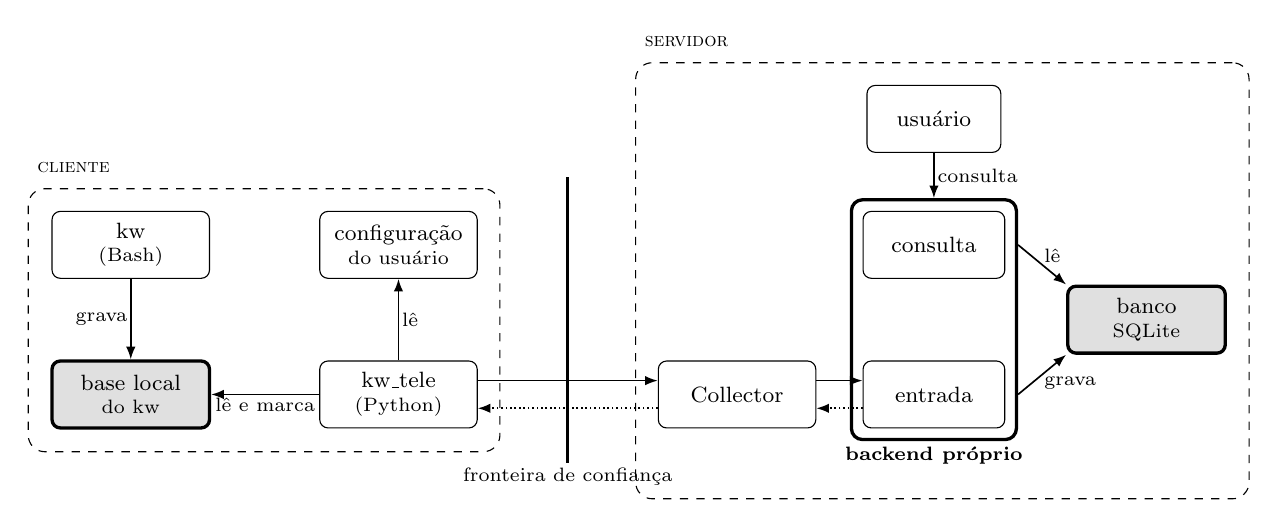
\begin{tikzpicture}[
    x=1cm, y=1cm,
    every node/.style={font=\footnotesize, align=center},
    peca/.style={draw, rounded corners=3pt, minimum width=2.0cm,
                 minimum height=0.85cm, inner sep=2pt, fill=white},
    dado/.style={peca, very thick, fill=black!12},
    lado/.style={draw, dashed, rounded corners=6pt, inner sep=8pt},
    rotulo/.style={font=\scriptsize\scshape, anchor=south west},
    seta/.style={-{Latex[length=1.6mm]}, semithick},
    volta/.style={-{Latex[length=1.6mm]}, semithick, densely dotted},
    nota/.style={font=\scriptsize, inner sep=1pt},
  ]
  \node[peca] (kw) at (0, 2.5) {kw\\[-1pt]{\scriptsize(Bash)}};
  \node[dado] (db) at (0, 0.6) {base local\\[-1pt]{\scriptsize do kw}};
  \node[peca] (tele) at (3.4, 0.6) {kw\_tele\\[-1pt]{\scriptsize(Python)}};
  \node[peca] (cfg) at (3.4, 2.5) {configuração\\[-1pt]{\scriptsize do usuário}};

  \node[peca] (col) at (7.7, 0.6) {Collector};
  \node[peca, minimum width=1.8cm] (ent) at (10.2, 0.6) {entrada};
  \node[peca, minimum width=1.8cm] (cons) at (10.2, 2.5) {consulta};
  \node[draw, very thick, rounded corners=4pt, inner sep=4pt, fit=(ent)(cons)] (back) {};
  \node[nota, font=\scriptsize\bfseries, anchor=north] at ([yshift=-1pt]back.south) {backend próprio};
  \node[dado] (sql) at (12.9, 1.55) {banco\\[-1pt]{\scriptsize SQLite}};
  \node[peca, minimum width=1.7cm] (pesq) at (10.2, 4.1) {usuário};

  \node[lado, fit=(kw)(db)(tele)(cfg)] (maq) {};
  \coordinate (fundo) at ([yshift=-0.45cm]back.south);
  \node[lado, fit=(col)(back)(sql)(pesq)(fundo)] (rec) {};
  \node[rotulo] at ([yshift=2pt]maq.north west) {cliente};
  \node[rotulo] at ([yshift=2pt]rec.north west) {servidor};

  \path (maq.east) -- coordinate[midway] (fx) (rec.west);
  \draw[very thick] ([yshift=4pt]fx |- maq.north) -- ([yshift=-4pt]fx |- maq.south)
    node[below, nota] {fronteira de confiança};

  \draw[seta] (kw) -- node[nota, left] {grava} (db);
  \draw[seta] (tele) -- node[nota, below] {lê e marca} (db);
  \draw[seta] (tele) -- node[nota, right] {lê} (cfg);

  \draw[seta] ([yshift=5pt]tele.east) -- ([yshift=5pt]col.west);
  \draw[seta] ([yshift=5pt]col.east) -- ([yshift=5pt]ent.west);
  \draw[volta] ([yshift=-5pt]ent.west) -- ([yshift=-5pt]col.east);
  \draw[volta] ([yshift=-5pt]col.west) -- ([yshift=-5pt]tele.east);

  \draw[seta] (ent.east -| back.east) -- node[nota, below right, inner sep=0.5pt] {grava} (sql.south west);
  \draw[seta] (cons.east -| back.east) -- node[nota, above right, inner sep=0.5pt] {lê} (sql.north west);
  \draw[seta] (pesq.south) -- node[nota, right] {consulta} (pesq.south |- back.north);
\end{tikzpicture}
}
  \caption{Caminho dos dados, da máquina de quem usa o kw até a consulta. A
    linha vertical marca a fronteira de confiança; a seta pontilhada é a
    confirmação, que volta pelo mesmo caminho depois que o backend próprio
    grava os registros.}
  \label{fig:arquitetura-caminho}
\end{figure}

Do lado do cliente ficam dois componentes. O próprio kw registra as
execuções e, antes de cada comando, decide se pergunta pelo consentimento ou
se dispara um envio em segundo plano, que nunca faz o comando esperar. O
kw\_tele, escrito em Python só com a biblioteca padrão, lê o banco do kw,
reduz a granularidade do tempo, tira os campos que o usuário escolheu não
enviar, monta o registro OTLP, envia e marca o que foi entregue. A
Seção~\ref{sec:cliente} trata dos dois.

Do lado do servidor ficam os outros. O Collector é o receptor de OTLP já
pronto, só configurado: limita o uso de memória e repassa os registros ao
backend, sem filtrar por atributo. O backend próprio separa os registros, põe à
parte os malformados e grava os demais, sem repetir o que já tinha. O backend
também responde às consultas, por rotas só de leitura: umas dizem que tipos de
registro e que atributos existem nos dados, e outra agrupa os registros por
qualquer um desses atributos. Os dois componentes estão na
Seção~\ref{sec:backend}, e a consulta, na Seção~\ref{sec:consulta}.

A fronteira de confiança, a linha entre o que o usuário controla e o que
outros recebem, é a máquina de quem usa o kw. Do lado de dentro estão o banco
do kw, a configuração e o kw\_tele, que roda como o próprio usuário. O único
ponto em que o dado cruza a fronteira é o envio do kw\_tele ao Collector; dali em diante, tudo fica do lado do servidor, e nenhum componente ali sabe o
que cada usuário escolheu.

Por isso, a privacidade é aplicada no cliente, antes de o dado sair da
máquina: o opt-in, a exclusão dos campos que o usuário escolher, a granularidade
de semana do tempo e o identificador aleatório de cada instalação. O Collector
não filtra nada por campo e supõe que o que chega foi consentido. O backend
reduz de novo a granularidade do tempo no que recebe, para que a regra valha
também contra um cliente antigo ou de outra origem. Os detalhes de cada
mecanismo estão no Capítulo~\ref{cap:privacidade}.

As duas pontas têm bancos separados. O do kw segue o esquema do kw; o do
backend é genérico e não sabe nada sobre o kw, porque guarda os atributos que
chegam sem conhecê-los de antemão. Essa separação é o que sustenta a
extensibilidade do sistema, discutida na Seção~\ref{sec:extensibilidade}.

\section{O banco local do kw}
\label{sec:banco-local}

Todo dado que sai da máquina começa no banco do kw
(Seção~\ref{sec:base-local}). O kw grava cada uso como um evento, uma linha
da tabela de eventos com identificador, data e hora, e o resto do que se sabe
sobre aquele uso fica em outras tabelas, ligadas ao evento. Este texto chama
de \emph{tabela de extensão} uma tabela cuja chave aponta, como chave
estrangeira, para o identificador do evento, e que acrescenta informação a
ele; a de execuções é a que o kw já tinha. Os nomes de comando e de estado não
ficam por extenso nessas tabelas: ficam como um número que aponta para uma
\emph{tabela de nomes}. O banco tem um dono só: o kw cria e muda o esquema, e
o kw\_tele apenas lê os eventos e atualiza neles uma marca de envio.

As três propriedades do esquema apresentadas na Seção~\ref{sec:base-local}
não atrapalham o \texttt{kw report}, mas pesam quando o dado sai da máquina,
e a elas se soma uma quarta: o banco não tinha onde registrar que um evento já
foi enviado. Um identificador reaproveitado faria um evento novo passar por um
já enviado. A hora local sem fuso não é o instante absoluto que o OTLP espera.
Sem versão do esquema, nada garante que uma instalação existente tenha uma
coluna nova. E, sem estado de exportação, não havia como evitar reenviar e
contar duas vezes o que já tinha saído. A Tabela~\ref{tab:esquema} resume o
efeito de cada uma e o que foi feito.

\begin{table}[!ht]
  \centering
  \footnotesize
  \setlength{\tabcolsep}{4pt}
  \begin{threeparttable}
    \caption{O que cada propriedade do esquema do kw faz com a exportação e o
      que foi feito.}
    \label{tab:esquema}
    \begin{tabular}{@{}>{\raggedright\arraybackslash}p{4.0cm}
                      >{\raggedright\arraybackslash}p{3.8cm}
                      >{\raggedright\arraybackslash}p{6.4cm}@{}}
      \toprule
      Propriedade do esquema & Efeito na exportação & O que foi feito \\
      \midrule
      identificador por ordem de inserção, sem garantia de não reaproveitamento
        & um evento novo poderia passar por um já enviado
        & contornado: a marca confere identificador e conteúdo, e a chave de
          repetição usa o identificador. Proposta: impedir o reaproveitamento,
          o que exige recriar a tabela \\
      \addlinespace
      data e hora em texto, na hora local, sem fuso
        & a virada da semana fica incerta
        & contornado pela granularidade de semana. Proposta: uma coluna com o
          instante em UTC \\
      \addlinespace
      sem versão do esquema
        & uma coluna nova depende de verificação no ponto de uso
        & feito o mínimo: uma verificação antes do envio, que só acrescenta o que
          falta. Proposta: versão do esquema e uma guarda de migração \\
      \addlinespace
      sem estado de exportação
        & reenvio e contagem dupla
        & feito: uma coluna no evento, com um índice, marca o que foi enviado \\
      \bottomrule
    \end{tabular}
    \begin{tablenotes}
      \footnotesize
      \item Justificativas na Seção~\ref{sec:banco-local}.
    \end{tablenotes}
  \end{threeparttable}
\end{table}


A mudança nas tabelas que já existiam é uma só, e aditiva: uma coluna no evento
que diz se ele está pendente, se ficou de fora do envio por ser anterior ao
consentimento ou em que momento foi enviado. Ela mora no banco do kw, junto com
os dados de uso que descreve, e não num arquivo à parte, e é a própria fila de
envio do kw\_tele (Seção~\ref{sec:cliente}). Como o esquema não tem versão, uma
verificação feita antes de perguntar o consentimento, antes de cada envio e nos
comandos de telemetria acrescenta a coluna aos bancos já instalados quando ela
falta. Nenhuma tabela, coluna ou \textit{view} existente foi alterada. A lista
de módulos entrou como uma tabela de extensão nova, e o kw grava o evento e a
sua linha de extensão juntos, para que a linha nunca fique sem evento
(Seção~\ref{sec:extensibilidade}). Essas mudanças, com o disparador de envio
(Seção~\ref{sec:cliente}), estão num ramo do \textit{fork} do kw usado neste
trabalho e não foram propostas ao projeto.

Três mudanças ficam como proposta. A primeira é uma coluna com o instante do
evento em UTC, ao lado da data e da hora atuais, o que resolveria a virada da
semana e a ordenação, e é defensável como correção isolada. A segunda é
impedir o reaproveitamento do identificador, o que exige recriar a tabela de
eventos. A terceira é versionar o esquema, com uma guarda de migração. O
trabalho parou na mudança mínima porque, sem versionamento, alterar a tabela
de eventos exigiria antes construir a infraestrutura de migração e mexeria em
funções do kw que dependem das \textit{views} atuais, o que, na leitura deste
trabalho, não se justifica só pela telemetria. Enquanto isso, o cliente e o
backend contornam as propriedades: a marca de envio confere o identificador, a
data e a hora do evento, a chave de repetição do backend usa o identificador,
e a granularidade de semana torna o fuso relevante só perto da virada da
semana.

\section{O cliente}
\label{sec:cliente}

O cliente tem duas metades. Uma é pequena, fica dentro do kw, é escrita em
Bash e roda antes de cada comando só para decidir se é preciso fazer alguma
coisa. A outra é um programa separado, o kw\_tele, escrito em Python, que lê
os eventos, prepara o registro e o envia. A divisão segue de uma regra
simples: o que roda em todo comando tem de custar quase nada e nunca falhar, e
montar JSON e falar HTTP com confirmação de entrega é trabalho que o Bash não
faz bem. O kw\_tele é chamado pelo kw do mesmo modo que outras ferramentas
externas que ele já usa, a exemplo do \texttt{patch-hub}
(Seção~\ref{sec:kw-o-que-e}).

Do lado do kw, o registro de uso continua como era: cada execução vira um
evento no banco local, por um único ponto de escrita
(Seção~\ref{sec:funcionalidades}). O que muda é que cada evento ganha uma marca de envio
(Seção~\ref{sec:banco-local}) e que uma verificação curta, o disparador de
envio, roda antes de cada comando. O
disparador faz uma sequência de perguntas (Figura~\ref{fig:disparador}): se o
comando é o próprio \texttt{kw telemetry}, que fica de fora; se o kw\_tele
está instalado; qual é o consentimento; e, com o consentimento dado, se o
comando é dos que registram uso e se já é hora de enviar. Enquanto o usuário
não responde, a pergunta de consentimento vem antes de qualquer outro comando,
inclusive os de ajuda e de versão, que não registram uso.

O disparador decide que é hora de enviar quando venceu o intervalo desde o
último envio bem-sucedido ou quando há eventos pendentes
demais, para que quem usa muito o kw não acumule uma fila grande; entre um
disparo e outro há também um intervalo de tempo mínimo, que cresce quando os
envios falham. O Go faz algo parecido, ao enviar seus relatórios uma vez por semana
(Seção~\ref{sec:precedentes}).

\begin{figure}[!ht]
  \centering
  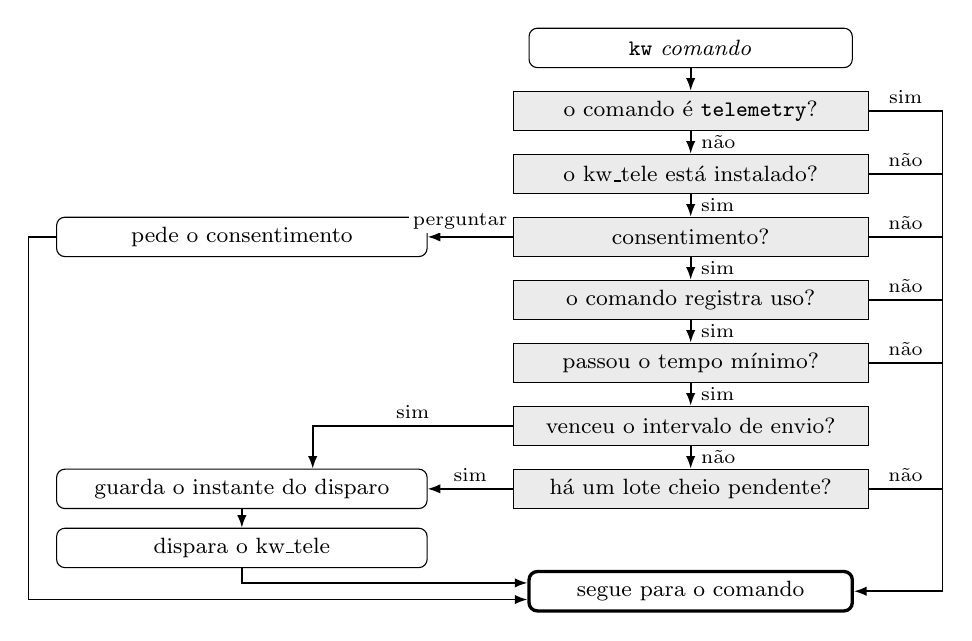
\begin{tikzpicture}[
    x=1cm, y=1cm,
    every node/.style={font=\footnotesize, align=center},
    passo/.style={draw, rounded corners=3pt, minimum height=0.5cm,
                  inner sep=1.5pt, fill=white, text width=4.0cm},
    pergunta/.style={draw, minimum height=0.5cm, inner sep=1.5pt,
                  fill=black!8, text width=4.4cm},
    fim/.style={passo, very thick},
    seta/.style={-{Latex[length=1.6mm]}, semithick},
    nota/.style={font=\scriptsize, inner sep=1.5pt, fill=white},
  ]
  \node[passo] (ini) at (0, 0) {\texttt{kw} \textit{comando}};
  \node[pergunta] (d1) at (0, -0.8) {o comando é \texttt{telemetry}?};
  \node[pergunta] (d2) at (0, -1.6) {o kw\_tele está instalado?};
  \node[pergunta] (d3) at (0, -2.4) {consentimento?};
  \node[pergunta] (d4) at (0, -3.2) {o comando registra uso?};
  \node[pergunta] (d5) at (0, -4.0) {passou o tempo mínimo?};
  \node[pergunta] (d6) at (0, -4.8) {venceu o intervalo de envio?};
  \node[pergunta] (d7) at (0, -5.6) {há um lote cheio pendente?};
  \node[fim] (segue) at (0, -6.9) {segue para o comando};

  \node[passo, text width=4.6cm] (ask) at (-5.7, -2.4) {pede o consentimento};
  \node[passo, text width=4.6cm] (marca) at (-5.7, -5.6) {guarda o instante do disparo};
  \node[passo, text width=4.6cm] (lanca) at (-5.7, -6.35) {dispara o kw\_tele};

  \draw[seta] (ini) -- (d1);
  \draw[seta] (d1) -- node[nota, right=2pt] {não} (d2);
  \draw[seta] (d2) -- node[nota, right=2pt] {sim} (d3);
  \draw[seta] (d3) -- node[nota, right=2pt] {sim} (d4);
  \draw[seta] (d4) -- node[nota, right=2pt] {sim} (d5);
  \draw[seta] (d5) -- node[nota, right=2pt] {sim} (d6);
  \draw[seta] (d6) -- node[nota, right=2pt] {não} (d7);

  \def\trilho{3.2}
  \draw[semithick] (d1.east) -- node[nota, above=1pt] {sim} (d1.east -| {(\trilho,0)});
  \foreach \d in {d2, d3, d4, d5, d7} {
    \draw[semithick] (\d.east) -- node[nota, above=1pt] {não} (\d.east -| {(\trilho,0)});
  }
  \draw[seta] (d1.east -| {(\trilho,0)}) -- (segue.east -| {(\trilho,0)}) -- (segue.east);

  \draw[seta] (d3.west) -- node[nota, above=1pt, pos=0.62] {perguntar} (ask.east);
  \draw[seta] (ask.west) -- ++(-0.35, 0) |- ([yshift=-3pt]segue.west);

  \draw[seta] (d6.west) -- node[nota, above=1pt] {sim} ([xshift=0.9cm]d6.west -| marca.north) -- ([xshift=0.9cm]marca.north);
  \draw[seta] (d7.west) -- node[nota, above=1pt] {sim} (marca.east);
  \draw[seta] (marca) -- (lanca);
  \draw[seta] (lanca.south) |- ([yshift=3pt]segue.west);
\end{tikzpicture}

  \caption{O que o disparador decide antes de cada comando do kw. Toda saída
    termina no comando; só a pergunta do consentimento espera o usuário, e o
    envio corre em segundo plano.}
  \label{fig:disparador}
\end{figure}

O consentimento é opt-in: o padrão é não enviar nada. O usuário responde a
uma pergunta no terminal, na qual também decide se os eventos gravados antes
da resposta vão junto, pode excluir campos do envio e pode mudar de ideia a
qualquer momento. Tudo isso é aplicado no cliente
(Seção~\ref{sec:arquitetura}), e as respostas possíveis e o que cada uma faz
estão no Capítulo~\ref{cap:privacidade}. O único momento em que o disparador espera o usuário é a pergunta de
consentimento, e só quando há um terminal para respondê-la; as demais
verificações são consultas locais curtas; em todos os casos, ele termina deixando o comando
seguir, e um problema na telemetria nunca impede um comando do kw de rodar.

Quando é hora de enviar, o disparador não envia. Ele dispara o kw\_tele em
segundo plano, com prazo, desligado do terminal, e deixa o comando seguir; o
comando não espera pelo envio. Um backend parado não pode segurar, por
exemplo, uma compilação do kernel. Uma falha no envio vira um estado guardado
na máquina, e não um erro do comando, e o disparador o lê na vez seguinte.
Como não há processo residente, também não há relógio: o envio acontece no
primeiro comando elegível depois de vencido o intervalo, e não numa hora
marcada.

Uma execução do kw\_tele segue um fluxo linear
(Figura~\ref{fig:kwtele-execucao}). Ele confere o consentimento a cada lote,
lê o esquema do banco do kw para saber que tabelas estendem o evento e
seleciona os eventos pendentes em lotes. Para cada evento, reduz a
granularidade do tempo, tira os campos que o usuário excluiu e monta o
registro OTLP (Seção~\ref{sec:mapeamento}); então envia o lote e marca as
linhas só depois de o backend confirmar que as gravou
(Seção~\ref{sec:backend}). A fila de envio é a própria marca no banco do kw, e
não uma fila na memória do programa. Se o backend recusa um lote pelo
conteúdo, o kw\_tele divide o lote até isolar a linha recusada, que fica
pendente para a próxima execução, e segue com as demais; ao fim, a execução
conta como falha, para que a linha seja tentada de novo; qualquer outra falha
interrompe a execução, que é refeita numa vez seguinte. O programa não conhece
as colunas de antemão: ele as lê do banco, o que é a base do argumento da
Seção~\ref{sec:extensibilidade}.

\begin{figure}[!ht]
  \centering
  \resizebox{\textwidth}{!}{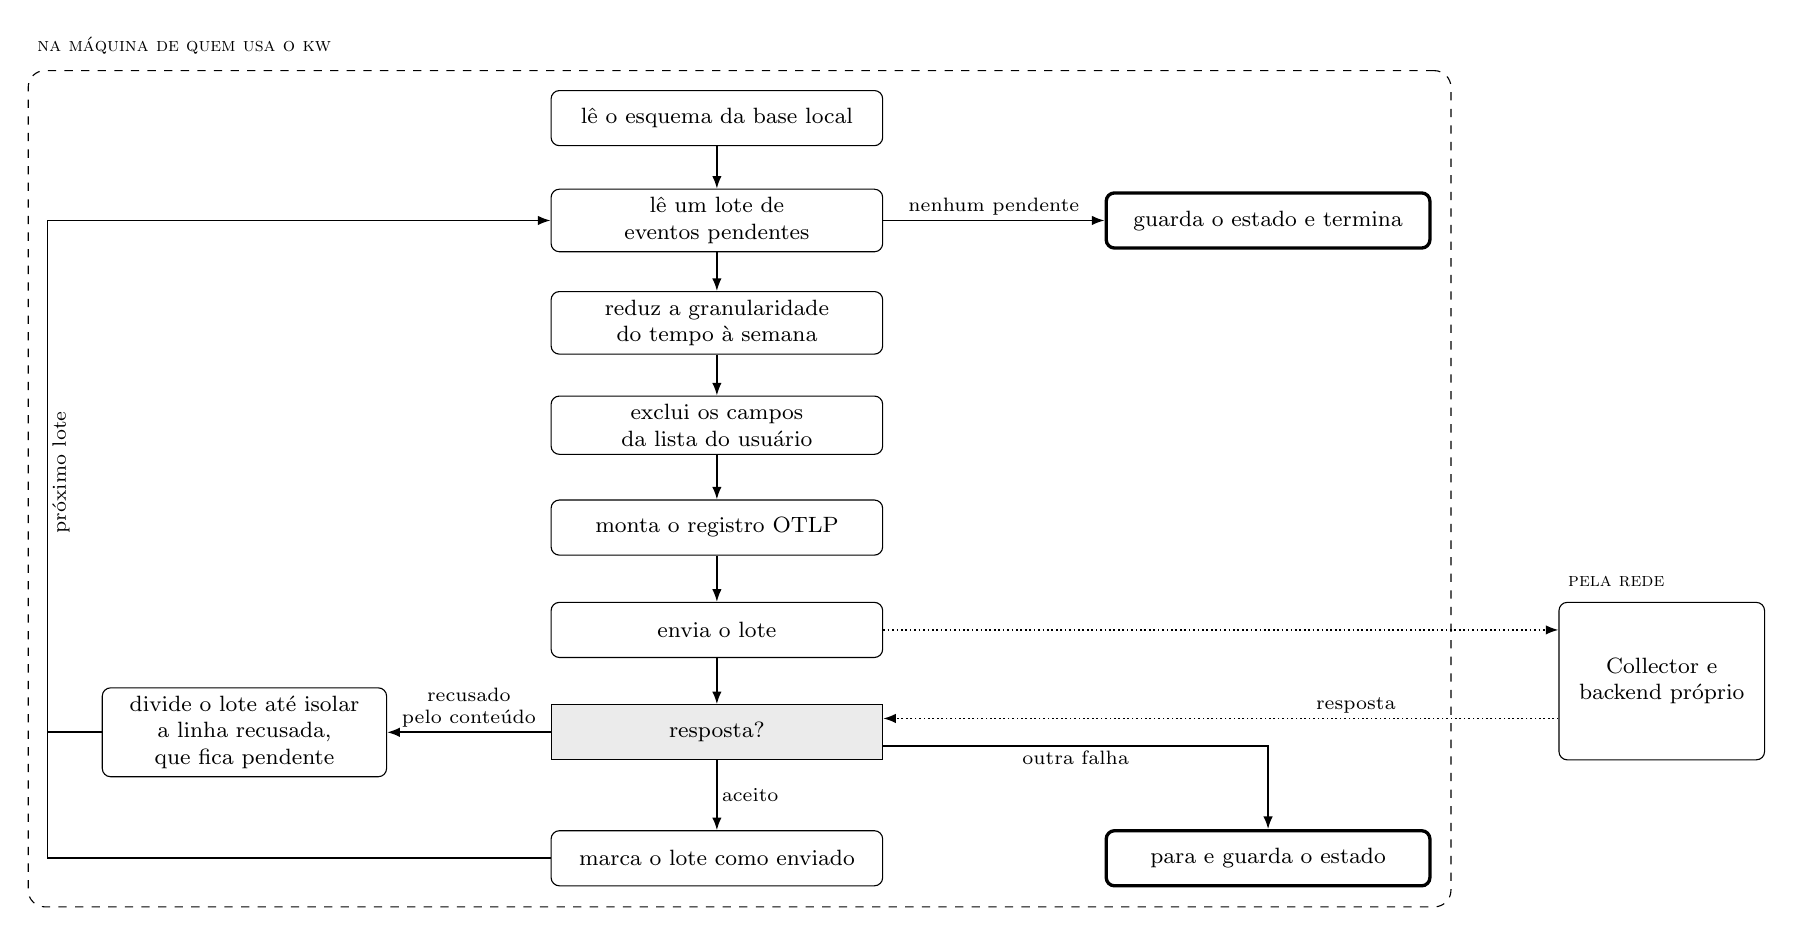
\begin{tikzpicture}[
    x=1cm, y=1cm,
    every node/.style={font=\footnotesize, align=center},
    passo/.style={draw, rounded corners=3pt, minimum height=0.7cm,
                  inner sep=3pt, fill=white, text width=4.0cm},
    pergunta/.style={draw, minimum height=0.7cm, inner sep=3pt,
                  fill=black!8, text width=4.0cm},
    fim/.style={passo, very thick, text width=3.9cm},
    lado/.style={draw, dashed, rounded corners=6pt, inner sep=7pt},
    rotulo/.style={font=\scriptsize\scshape, anchor=south west},
    seta/.style={-{Latex[length=1.6mm]}, semithick},
    rede/.style={-{Latex[length=1.6mm]}, semithick, densely dotted},
    nota/.style={font=\scriptsize, inner sep=1.5pt},
  ]
  \node[passo] (esq) at (0, 0) {lê o esquema da base local};
  \node[passo] (pend) at (0, -1.3) {lê um lote de\\eventos pendentes};
  \node[passo] (tempo) at (0, -2.6) {reduz a granularidade do tempo à semana};
  \node[passo] (excl) at (0, -3.9) {exclui os campos da lista do usuário};
  \node[passo] (monta) at (0, -5.2) {monta o registro OTLP};
  \node[passo] (envia) at (0, -6.5) {envia o lote};
  \node[pergunta] (resp) at (0, -7.8) {resposta?};
  \node[passo] (marca) at (0, -9.4) {marca o lote como enviado};

  \node[fim] (termina) at (7.0, -1.3) {guarda o estado e termina};
  \node[fim] (para) at (7.0, -9.4) {para e guarda o estado};
  \node[passo, text width=3.4cm] (divide) at (-6.0, -7.8)
    {divide o lote até isolar a linha recusada, que fica pendente};

  \coordinate (vl) at (-8.5, -4.5);
  \node[lado, fit=(esq)(marca)(termina)(para)(divide)(vl)] (maq) {};
  \node[rotulo] at ([yshift=2pt]maq.north west) {na máquina de quem usa o kw};

  \node[passo, text width=2.4cm, minimum height=2.0cm] (rec) at (12.0, -7.15)
    {Collector e\\backend próprio};
  \node[rotulo] at ([yshift=2pt]rec.north west) {pela rede};

  \draw[seta] (esq) -- (pend);
  \draw[seta] (pend) -- (tempo);
  \draw[seta] (tempo) -- (excl);
  \draw[seta] (excl) -- (monta);
  \draw[seta] (monta) -- (envia);
  \draw[seta] (envia) -- (resp);
  \draw[seta] (pend) -- node[nota, above] {nenhum pendente} (termina);

  \draw[rede] (envia.east) -- (envia.east -| rec.west);
  \draw[rede] ([yshift=5pt]resp.east -| rec.west) -- node[nota, above, pos=0.3] {resposta} ([yshift=5pt]resp.east);

  \draw[seta] (resp) -- node[nota, right] {aceito} (marca);
  \draw[seta] (resp.west) -- node[nota, above, align=center] {recusado\\pelo conteúdo} (divide.east);
  \draw[seta] ([yshift=-5pt]resp.east) -| node[nota, below, pos=0.25] {outra falha} (para.north);

  \def\volta{-8.5}
  \draw[seta] (marca.west) -- (\volta, -9.4) -- (\volta, -1.3) -- (pend.west);
  \draw[semithick] (divide.west) -- (\volta, -7.8);
  \node[nota, rotate=90, below] at (\volta, -4.5) {próximo lote};
\end{tikzpicture}
}
  \caption{Uma execução do kw\_tele. As setas pontilhadas atravessam a rede; um
    lote recusado pelo conteúdo é dividido até isolar a linha recusada, que fica
    pendente.}
  \label{fig:kwtele-execucao}
\end{figure}

Esse design decorre do que o kw é: uma ferramenta em Bash, que não deve ganhar
dependências pesadas, feita de comandos curtos, sem nada residente, e cuja
telemetria não pode atrasar nem quebrar um comando. Disso decorrem duas
escolhas. A primeira é não usar o SDK do OpenTelemetry no cliente. O SDK traz
instrumentação e convenções prontas, mas, no SDK de Python com processamento
em lote, quem envia não sabe se o envio chegou, e este design precisa marcar
cada linha como enviada só depois da confirmação; além disso, o SDK traria
dependências que o cliente evita. A comparação, com as fontes, está nas
Seções~\ref{sec:alternativas} e~\ref{sec:limites-otel}; o caminho síncrono do
SDK não foi avaliado.

A segunda escolha é usar o OTLP sobre HTTP com corpo JSON, e não sobre gRPC
com protobuf. O Python traz JSON e HTTP na biblioteca padrão e não traz gRPC
nem protobuf, e o corpo em JSON pode ser lido por quem quiser conferir o que
seria enviado. O preço é um corpo maior e as regras do JSON do OTLP,
discutidas na Seção~\ref{sec:limites-otel}. Na leitura deste trabalho, um
processo que roda por segundos também não se beneficiaria da conexão longa do
gRPC.

\section{Do evento do kw ao registro OTLP}
\label{sec:mapeamento}

Esta seção acompanha um evento do kw do momento em que ele é gravado até sair
da máquina como registro OTLP. O exemplo é uma compilação bem-sucedida com a
lista de módulos, a fonte acrescentada ao kw como demonstração
(Seção~\ref{sec:extensibilidade}). Quando o usuário compila o kernel, o kw grava
um evento: uma linha da tabela de eventos, com identificador, data e hora
(Seção~\ref{sec:base-local}). O resto do que se sabe sobre aquela compilação fica nas tabelas de extensão
do evento (Seção~\ref{sec:banco-local}). Aqui há duas. A da execução, com o comando, a duração e o estado em que
terminou, já existia no kw. A da lista de módulos, com a contagem e os nomes,
é a nova, acrescentada neste exemplo. O comando e o estado ficam como um número que aponta para uma tabela de nomes.

Na hora do envio, o kw\_tele não sabe de antemão que tabelas existem. Ele lê o
esquema do banco e acha as tabelas de extensão por essa chave estrangeira, de
modo que uma tabela nova ligada ao evento passa a ser enviada sem mudar o
cliente. Para cada evento pendente, junta a linha do evento com as linhas das
extensões que têm o mesmo identificador e troca cada número pelo nome
correspondente. Cada linha de extensão vira um registro OTLP, e um evento sem
extensão vira um registro só. Nem todo comando preenche todas as tabelas de
extensão: cada comando grava só as que lhe dizem respeito. Compilar o kernel ou
instalá-lo numa máquina de teste preenche a da execução e a dos módulos; listar
ou remover os kernels instalados, só a da execução; o \texttt{pomodoro}
preenche apenas a sua, de sessões de trabalho. O número de registros por evento
varia, portanto, com o comando. A compilação do exemplo vira, portanto, dois
registros com o mesmo identificador de evento
(Figura~\ref{fig:evento-registro}).

\begin{figure}[!ht]
  \centering
  \resizebox{\textwidth}{!}{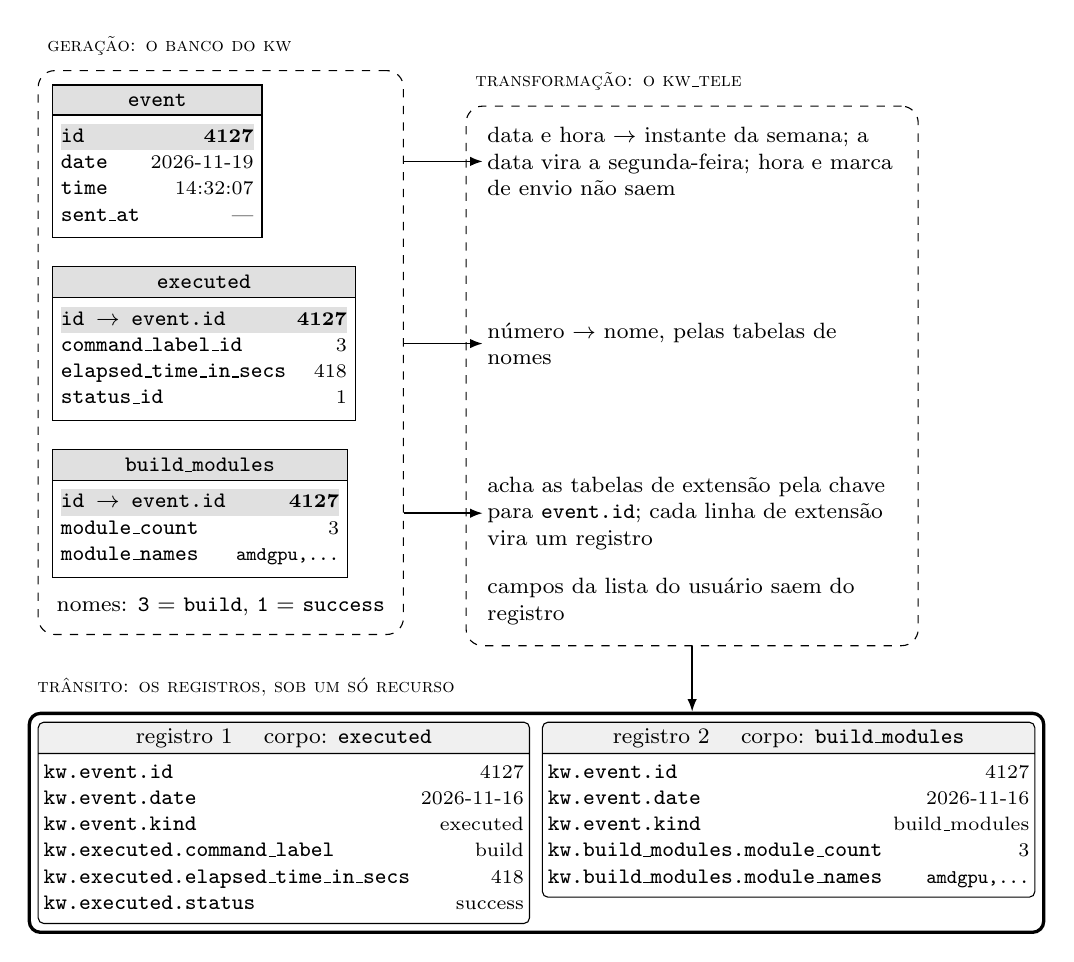
\begin{tikzpicture}[
    x=1cm, y=1cm,
    every node/.style={font=\footnotesize},
    tabela/.style={draw, rectangle split, rectangle split parts=2,
                   rectangle split part fill={black!12, white},
                   inner sep=3pt, font=\footnotesize},
    registro/.style={draw, rectangle split, rectangle split parts=2,
                   rectangle split part fill={black!6, white},
                   inner sep=2pt, font=\footnotesize, rounded corners=2pt},
    recurso/.style={draw, very thick, rounded corners=4pt, inner sep=3pt},
    coluna/.style={draw, dashed, rounded corners=6pt, inner sep=5pt},
    rotulo/.style={font=\scriptsize\scshape, anchor=south west},
    seta/.style={-{Latex[length=1.6mm]}, semithick},
    nota/.style={font=\footnotesize, align=left, inner sep=1.5pt},
  ]
  \providecommand{\kwcolunas}{}\renewcommand{\kwcolunas}[1]{%
    {\setlength{\tabcolsep}{0pt}\begin{tabular}{@{}l<{\hspace{0.45em}}@{}r@{}}#1\end{tabular}}}
  \providecommand{\kwcol}{}\renewcommand{\kwcol}[2]{\texttt{#1} & {\scriptsize #2}\\}
  \providecommand{\kwchave}{}\renewcommand{\kwchave}[2]{\rowcolor{black!12}\texttt{\textbf{#1}} & {\scriptsize\textbf{#2}}\\}

  \node[tabela, anchor=north west] (ev) at (0, 0) {%
    \texttt{event}
    \nodepart{two}
    \kwcolunas{\kwchave{id}{4127}\kwcol{date}{2026-11-19}\kwcol{time}{14:32:07}\kwcol{sent\_at}{---}}};

  \node[tabela, anchor=north west] (ex) at ([yshift=-0.35cm]ev.south west) {%
    \texttt{executed}
    \nodepart{two}
    \kwcolunas{\kwchave{id $\to$ event.id}{4127}\kwcol{command\_label\_id}{3}%
             \kwcol{elapsed\_time\_in\_secs}{418}\kwcol{status\_id}{1}}};

  \node[tabela, anchor=north west] (bm) at ([yshift=-0.35cm]ex.south west) {%
    \texttt{build\_modules}
    \nodepart{two}
    \kwcolunas{\kwchave{id $\to$ event.id}{4127}\kwcol{module\_count}{3}%
             \kwcol{module\_names}{\texttt{amdgpu,\dots}}}};

  \node[nota, anchor=north west] (nomes) at ([yshift=-0.2cm]bm.south west) {nomes: \texttt{3} = \texttt{build},
    \texttt{1} = \texttt{success}};


  \node[coluna, fit=(ev)(ex)(bm)(nomes)] (g) {};
  \node[rotulo] at ([yshift=2pt]g.north west) {geração: o banco do kw};

  \coordinate (tx) at ([xshift=1.0cm]g.east);
  \node[nota, anchor=west, text width=5.2cm] (t1) at (tx |- ev.center)
    {data e hora $\to$ instante da semana; a data vira a segunda-feira; hora e marca de envio não saem};
  \node[nota, anchor=west, text width=5.2cm] (t3) at (tx |- ex.center) {número $\to$ nome, pelas tabelas de nomes};
  \node[nota, anchor=west, text width=5.2cm] (t4) at (tx |- bm.center)
    {acha as tabelas de extensão pela chave para \texttt{event.id}; cada linha de extensão vira um registro};
  \node[nota, anchor=north west, text width=5.2cm] (t5) at ([yshift=-0.25cm]t4.south west)
    {campos da lista do usuário saem do registro};

  \node[coluna, fit=(t1)(t5), inner sep=6pt] (tr) {};
  \node[rotulo] at ([yshift=2pt]tr.north west) {transformação: o kw\_tele};

  \draw[seta] (ev.east -| g.east) -- (t1.west);
  \draw[seta] (ex.east -| g.east) -- (t3.west);
  \draw[seta] (bm.east -| g.east) -- (t4.west);

  \node[registro, anchor=north west] (r1) at ([yshift=-1.1cm]g.south west) {%
    registro 1 \quad corpo: \texttt{executed}
    \nodepart{two}
    \kwcolunas{\kwcol{kw.event.id}{4127}\kwcol{kw.event.date}{2026-11-16}%
             \kwcol{kw.event.kind}{executed}%
             \kwcol{kw.executed.command\_label}{build}%
             \kwcol{kw.executed.elapsed\_time\_in\_secs}{418}\kwcol{kw.executed.status}{success}}};

  \node[registro, anchor=north west] (r2) at ([xshift=0.15cm]r1.north east) {%
    registro 2 \quad corpo: \texttt{build\_modules}
    \nodepart{two}
    \kwcolunas{\kwcol{kw.event.id}{4127}\kwcol{kw.event.date}{2026-11-16}%
             \kwcol{kw.event.kind}{build\_modules}%
             \kwcol{kw.build\_modules.module\_count}{3}%
             \kwcol{kw.build\_modules.module\_names}{\texttt{amdgpu,\dots}}}};

  \node[recurso, fit=(r1)(r2)] (rq) {};
  \node[rotulo] at ([yshift=2pt]rq.north west) {trânsito: os registros, sob um só recurso};

  \draw[seta] (tr.south) -- (tr.south |- rq.north);
\end{tikzpicture}
}
  \caption{Um evento de compilação do kw virando dois registros OTLP, um por
    linha de extensão, sob um só recurso (Figura~\ref{fig:requisicao-otlp}). Valores
    ilustrativos.}
  \label{fig:evento-registro}
\end{figure}

Cada registro é montado com o que foi lido. O corpo traz o tipo do registro,
isto é, o nome da tabela de extensão, ou \enquote{event} quando não há
extensão, e o mesmo valor vai num atributo de tipo, para que a consulta agrupe
por tipo. Cada coluna vira um atributo cujo nome diz de onde ela veio:
\texttt{kw.event.<coluna>} para o evento e \texttt{kw.<tabela>.<coluna>} para a
extensão, como \texttt{kw.build\_modules.module\_count} no registro dos
módulos. A coluna que apontava para uma tabela de nomes sai com o nome, como o
comando, em \texttt{kw.executed.command\_label}. O identificador do evento vai
como atributo, porque o registro OTLP não tem identidade própria e o backend
precisa dele para reconhecer repetidos (Seção~\ref{sec:backend}). O nível de
severidade, o campo do modelo de \textit{logs} que classifica o registro como
informação, aviso ou erro, não tem equivalente no kw e sai com o valor neutro
de informação. A Tabela~\ref{tab:mapeamento} lista todos os campos.

\begin{table}[!ht]
  \centering
  \footnotesize
  \setlength{\tabcolsep}{4pt}
  \begin{threeparttable}
    \caption{Do evento do kw ao registro OTLP. As colunas de extensão não são
      fixas: o cliente as descobre no banco do kw a cada execução, e
      \texttt{executed} e \texttt{build\_modules} são exemplos.}
    \label{tab:mapeamento}
    \begin{tabular}{@{}>{\raggedright\arraybackslash}p{4.0cm}
                      >{\raggedright\arraybackslash}p{5.0cm}
                      >{\raggedright\arraybackslash}p{5.2cm}@{}}
      \toprule
      Origem no kw & Campo no registro OTLP & Tratamento \\
      \midrule
      \multicolumn{3}{@{}l}{\textit{Evento}} \\*
      \addlinespace[1pt]
      identificador do evento & \texttt{kw.event.id} & direto \\
      outra coluna do evento & \texttt{kw.event.}\textit{coluna} & direto \\
      data do evento & \texttt{kw.event.date} & vira a segunda-feira da semana \\
      hora do evento & --- & não enviada \\
      marca de envio & --- & não enviada \\
      data e hora do evento & \texttt{timeUnixNano} & instante da semana \\
      momento do envio & \texttt{observedTimeUnixNano} & instante da semana \\
      \midrule
      \multicolumn{3}{@{}l}{\textit{Extensões (descobertas no banco do kw)}} \\*
      \addlinespace[1pt]
      tabela de extensão & \texttt{body} e \texttt{kw.event.kind}
        & nome da tabela; \texttt{event} quando o evento não tem extensão;
          um registro por linha de extensão \\
      coluna da extensão & \texttt{kw.}\textit{tabela}\texttt{.}\textit{coluna} & direto \\
      coluna que aponta para uma tabela de nomes
        & \texttt{kw.}\textit{tabela}\texttt{.}\textit{coluna} sem o sufixo \texttt{\_id}
          (por exemplo, \texttt{kw.executed.command\_label})
        & o nome, no lugar do número \\
      \midrule
      \multicolumn{3}{@{}l}{\textit{Recurso (um por envio)}} \\*
      \addlinespace[1pt]
      instalação & \texttt{service.instance.id} & UUID aleatório, criado no opt-in \\
      kw e cliente
        & \texttt{service.name}, \texttt{service.version},
          \texttt{telemetry.sdk.name}, \texttt{.language}, \texttt{.version}
        & fixos, exceto as versões \\
      \midrule
      sem equivalente no kw & \texttt{severityNumber}, \texttt{severityText}
        & fixos: 9 e \texttt{INFO} \\
      \bottomrule
    \end{tabular}
    \begin{tablenotes}
      \footnotesize
      \item Justificativas na Seção~\ref{sec:mapeamento}.
    \end{tablenotes}
  \end{threeparttable}
\end{table}


O tempo é o único campo que muda de valor no caminho, e muda de propósito. No
kw, a data e a hora do evento estão em texto, no horário local e sem fuso. No
registro, o tempo vai com granularidade de semana: o campo do tempo do evento
leva o instante da semana em que ele ocorreu, um mesmo instante para toda a
semana, e o atributo da data passa a ser a segunda-feira daquela semana. A
hora não sai, e a marca de envio também não. O motivo é que o horário de
trabalho do usuário não sai da máquina (Capítulo~\ref{cap:privacidade}). A
redução não é configurável, e, quando a data guardada não é legível, o tempo
sai como desconhecido e a data não é enviada. O modelo de \textit{logs} prevê
nesse campo o instante em que o evento ocorreu \citep{otel_logs_data_model};
levar o instante da semana é um desvio deliberado, e um evento perto da virada
da semana em UTC pode cair na semana vizinha, limite retomado na
Seção~\ref{sec:banco-local}.

Os registros de um envio saem juntos, sob um recurso, a parte do documento OTLP
que diz quem os produziu: o serviço, a versão do kw, um identificador da
instalação e o nome, a linguagem e a versão do cliente, com os nomes de
atributo das convenções do OpenTelemetry, que marcam os quatro últimos como
estáveis \citep{otel_semconv_resource_v1_45_0}. O identificador da instalação é
aleatório, criado quando o usuário aceita enviar, como as convenções
recomendam \citep{otel_semconv_registry_service_v1_45_0}; ele serve para contar
instalações e separar os repetidos de cada uma, sem relação com o usuário ou a
máquina (Capítulo~\ref{cap:privacidade}). O cliente se identifica como
kw\_tele, e não pelo nome que as convenções reservam ao SDK oficial
\citep{otel_semconv_resource_v1_45_0}. Cada registro leva também o momento do
envio, como momento da observação, igualmente com granularidade de semana. O documento segue por HTTP, com corpo JSON, para o Collector
(Figura~\ref{fig:requisicao-otlp}). Cada evento vira um
registro de \textit{log} porque é um fato com tempo e atributos; contar e
agrupar fica para o backend.

\begin{figure}[!ht]
  \centering
  \begin{tikzpicture}[
    x=1cm, y=1cm,
    every node/.style={font=\footnotesize},
    linha/.style={anchor=west, inner sep=1pt, font=\footnotesize\ttfamily},
    titulo/.style={anchor=north west, inner sep=2pt, xshift=2pt, yshift=-1pt, font=\footnotesize\ttfamily\bfseries},
    nivel/.style={draw, rounded corners=3pt, inner sep=5pt},
    recolhido/.style={anchor=west, inner sep=1pt, font=\footnotesize\itshape, text=black!65},
    nota/.style={anchor=west, font=\scriptsize, align=left, inner sep=1.5pt, text width=4.8cm},
    liga/.style={semithick, densely dotted},
  ]
  \providecommand{\aspas}{}\renewcommand{\aspas}[1]{\textquotedbl{}#1\textquotedbl{}}

  \node[linha] (http) at (0, 0) {POST \textrm{\textit{<endpoint configurado>}}};
  \node[linha] (ct) at (0, -0.45) {Content-Type: application/json};

  \node[linha] (a1) at (0.9, -2.0) {service.name \textrm{=} \aspas{kworkflow}};
  \node[linha] (a2) at (0.9, -2.4) {service.version \textrm{=} \textrm{\textit{<versão do kw>}}};
  \node[linha] (a3) at (0.9, -2.8) {service.instance.id \textrm{=} \textrm{\textit{<UUID aleatório>}}};
  \node[linha] (a4) at (0.9, -3.2) {telemetry.sdk.name \textrm{=} \aspas{kw\_tele}};
  \node[linha] (a5) at (0.9, -3.6) {telemetry.sdk.language \textrm{=} \aspas{python}};
  \node[linha] (a6) at (0.9, -4.0) {telemetry.sdk.version \textrm{=} \textrm{\textit{<versão do kw\_tele>}}};
  \node[nivel, fit=(a1)(a6), inner ysep=9pt, yshift=6pt] (fres) {};
  \node[titulo] at (fres.north west) {resource.attributes};

  \node[linha] (sc) at (1.3, -5.25) {scope \textrm{=} \{name: \aspas{kw\_tele}, version\}};
  \node[linha] (r1) at (1.7, -6.25) {timeUnixNano, observedTimeUnixNano};
  \node[linha] (r2) at (1.7, -6.65) {severityNumber \textrm{=} 9};
  \node[linha] (r2b) at (1.7, -7.05) {severityText \textrm{=} \aspas{INFO}};
  \node[linha] (r3) at (1.7, -7.45) {body.stringValue \textrm{=} \textrm{\textit{<tipo>}}};
  \node[recolhido] (r4) at (1.7, -7.85) {attributes: \texttt{kw.event.*}, \texttt{kw.}\textit{<tabela>}\texttt{.*}};
  \node[recolhido] (r4b) at (1.7, -8.2) {(Figura~\ref{fig:evento-registro})};
  \node[nivel, fit=(r1)(r4b), inner ysep=9pt, yshift=6pt] (frec) {};
  \node[titulo] at (frec.north west) {logRecords[0]};
  \node[recolhido] (r5) at (1.3, -9.0) {logRecords[1], \dots};
  \node[nivel, fit=(sc)(frec)(r5), inner ysep=9pt, yshift=6pt] (fsl) {};
  \node[titulo] at (fsl.north west) {scopeLogs[0]};

  \node[nivel, very thick, fit=(fres)(fsl), inner ysep=10pt, yshift=7pt] (frl) {};
  \node[titulo] at (frl.north west) {resourceLogs[0]};

  \coordinate (col) at ([xshift=0.6cm]frl.east);
  \node[nota] (n0) at ([yshift=-0.2cm]col |- http) {a requisição: JSON, sem compressão,\\ao endpoint do Collector\\(o padrão termina em \texttt{/v1/logs})};
  \node[nota] (n1) at (col |- a1) {\textbf{resource}: uma vez por requisição; quem produziu os dados};
  \node[nota] (n2) at (col |- a3) {o identificador da instalação: aleatório, criado ao aceitar};
  \node[nota] (n3) at ([yshift=0.15cm]col |- sc) {\textbf{scope}: o cliente que montou\\os registros};
  \node[nota] (n4) at ([yshift=-0.3cm]col |- r1) {\textbf{logRecords}: um por linha\\de extensão; os dois tempos vão na\\granularidade de semana: o do\\evento e o do envio};
  \node[nota] (n5) at ([yshift=-0.75cm]col |- r3) {o corpo é o tipo do registro (o nome da tabela)};

  \draw[liga] (a1.east) -- (n1.west);
  \draw[liga] (a3.east) -- (n2.west);
  \draw[liga] (sc.east) -- (sc.east -| n3.west);
  \draw[liga] (r1.east) -| ([xshift=-0.3cm]n4.west) -- (n4.west);
  \draw[liga] (r3.east) -| ([xshift=-0.3cm]n5.west) -- (n5.west);
\end{tikzpicture}

  \caption{Uma requisição OTLP decomposta. Os atributos de cada registro estão
    na Figura~\ref{fig:evento-registro}.}
  \label{fig:requisicao-otlp}
\end{figure}

Na tradução, o evento virou o registro, cada coluna virou um atributo e a
tabela virou o tipo; pediram adaptação o tempo, as colunas de nomes, o
identificador do evento e o nível de severidade. O que o kw não guarda, o fuso
e a versão do esquema, e o identificador que pode ser reaproveitado são o
assunto da Seção~\ref{sec:banco-local}.

\section{O Collector e o backend próprio}
\label{sec:backend}

O Collector recebe, processa e repassa registros, mas não os guarda num banco
de dados. A distribuição usada, a principal, na versão 0.121.0, não traz
exportador para banco: os seus exportadores enviam a outro receptor, a um
arquivo ou a sistemas de métricas e de mensagens
\citep{otelcol_releases_manifest_0_121_0}. Exportadores para bancos, como o do
ClickHouse, existem só na distribuição \textit{contrib}, em estágio beta para
\textit{logs} \citep{otelcol_contrib_clickhouse_metadata_0_121_0}, e nenhum
grava em SQLite. Por isso este trabalho pôs um backend próprio depois do
Collector, e a divisão de papéis ficou assim: o Collector é a parte exposta
aos clientes, que recebe o protocolo e se protege de picos de carga; o backend
fica atrás dele, separa, guarda e confirma, e serve a consulta
(Seção~\ref{sec:consulta}). Na leitura deste trabalho, é essa divisão que
deixa ao código escrito aqui só o que é específico do caminho.

O Collector é usado como vem, só por configuração
(Figura~\ref{fig:collector}): um receptor de OTLP sobre
HTTP, um limite de uso de memória, um processador que só acrescenta um
atributo de marcação e um exportador que repassa os registros ao backend
próprio. É esse reuso que motivou a escolha do OpenTelemetry
(Seção~\ref{sec:criterios}): o trabalho não precisou escrever o receptor
voltado aos clientes nem a proteção contra picos de carga. O limite de memória
vem antes de tudo e recusa o excesso antes de processá-lo, e o cliente trata
essa recusa como passageira, deixando as linhas para uma próxima vez. O
Collector não agrupa registros em lote nem guarda fila, por uma razão
explicada adiante, e não filtra nada por campo: ele supõe que o que chega já
foi consentido (Seção~\ref{sec:arquitetura}).

\begin{figure}[!ht]
  \centering
  \resizebox{\textwidth}{!}{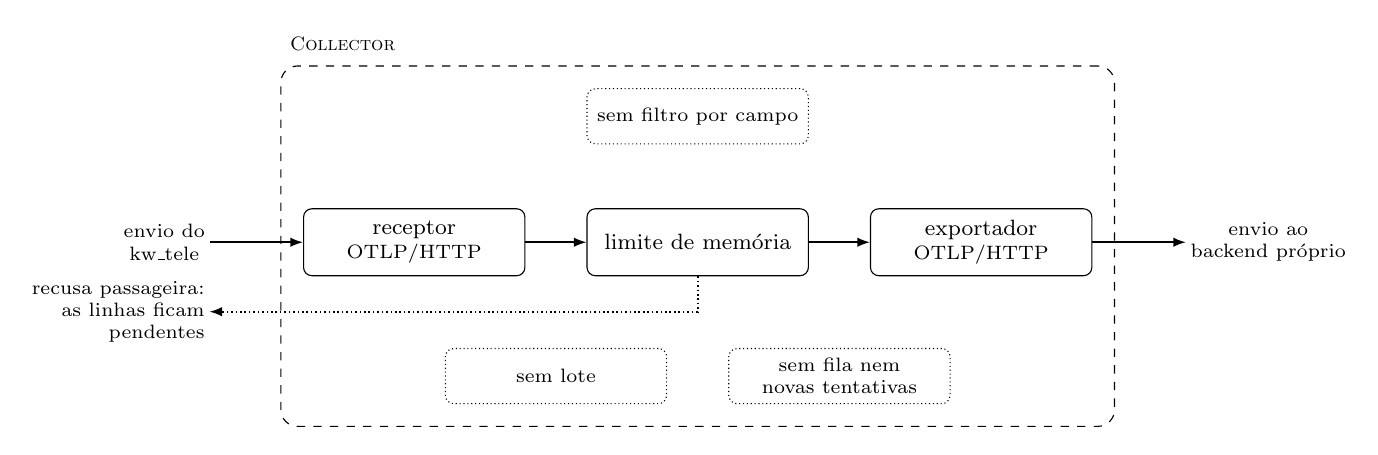
\begin{tikzpicture}[
    x=1cm, y=1cm,
    every node/.style={font=\footnotesize, align=center},
    peca/.style={draw, rounded corners=3pt, minimum height=0.85cm,
                 inner sep=3pt, fill=white, text width=2.6cm},
    ausente/.style={draw, densely dotted, rounded corners=3pt, minimum height=0.7cm,
                 inner sep=3pt, text width=2.6cm, font=\scriptsize},
    lado/.style={draw, dashed, rounded corners=6pt, inner sep=8pt},
    rotulo/.style={font=\scriptsize\scshape, anchor=south west},
    seta/.style={-{Latex[length=1.6mm]}, semithick},
    volta/.style={-{Latex[length=1.6mm]}, semithick, densely dotted},
    nota/.style={font=\scriptsize, inner sep=1.5pt},
  ]
  \node[peca] (rec) at (0, 0) {receptor\\[-1pt]{\scriptsize OTLP/HTTP}};
  \node[peca] (mem) at (3.6, 0) {limite de memória};
  \node[peca] (exp) at (7.2, 0) {exportador\\[-1pt]{\scriptsize OTLP/HTTP}};

  \node[ausente] (a1) at (1.8, -1.7) {sem lote};
  \node[ausente] (a2) at (5.4, -1.7) {sem fila nem novas tentativas};
  \node[ausente] (a3) at (3.6, 1.6) {sem filtro por campo};

  \node[lado, fit=(rec)(exp)(a1)(a2)(a3)] (col) {};
  \node[rotulo] at ([yshift=2pt]col.north west) {Collector};

  \node[nota, anchor=east] (in) at (-2.6, 0) {envio do\\kw\_tele};
  \node[nota, anchor=west] (out) at (9.8, 0) {envio ao\\backend próprio};

  \draw[seta] (in.east) -- (rec.west);
  \draw[seta] (rec) -- (mem);
  \draw[seta] (mem) -- (exp);
  \draw[seta] (exp.east) -- (out.west);

  \draw[volta] (mem.south) -- ++(0, -0.45) coordinate (m1) -- (m1 -| in.east)
    node[nota, left, align=right] {recusa passageira:\\as linhas ficam\\pendentes};
\end{tikzpicture}
}
  \caption{Dentro do Collector, no caminho dos registros. O que está
    pontilhado não existe neste caminho.}
  \label{fig:collector}
\end{figure}

O backend próprio entende só a pequena parte do OTLP sobre HTTP de que o
caminho precisa, que é receber registros de \textit{log}. Ele separa o corpo da
requisição que o Collector repassa em registros
(Figura~\ref{fig:backend-entrada}), e o que não se encaixa no formato vai para um
armazenamento à parte, junto com o motivo, sem derrubar o resto do lote. O
conteúdo nunca é motivo para recusar uma requisição: se fosse, cada registro
malformado faria o cliente dividir o lote até isolá-lo e deixá-lo pendente,
para recusá-lo de novo a cada tentativa.

\begin{figure}[!ht]
  \centering
  \resizebox{\textwidth}{!}{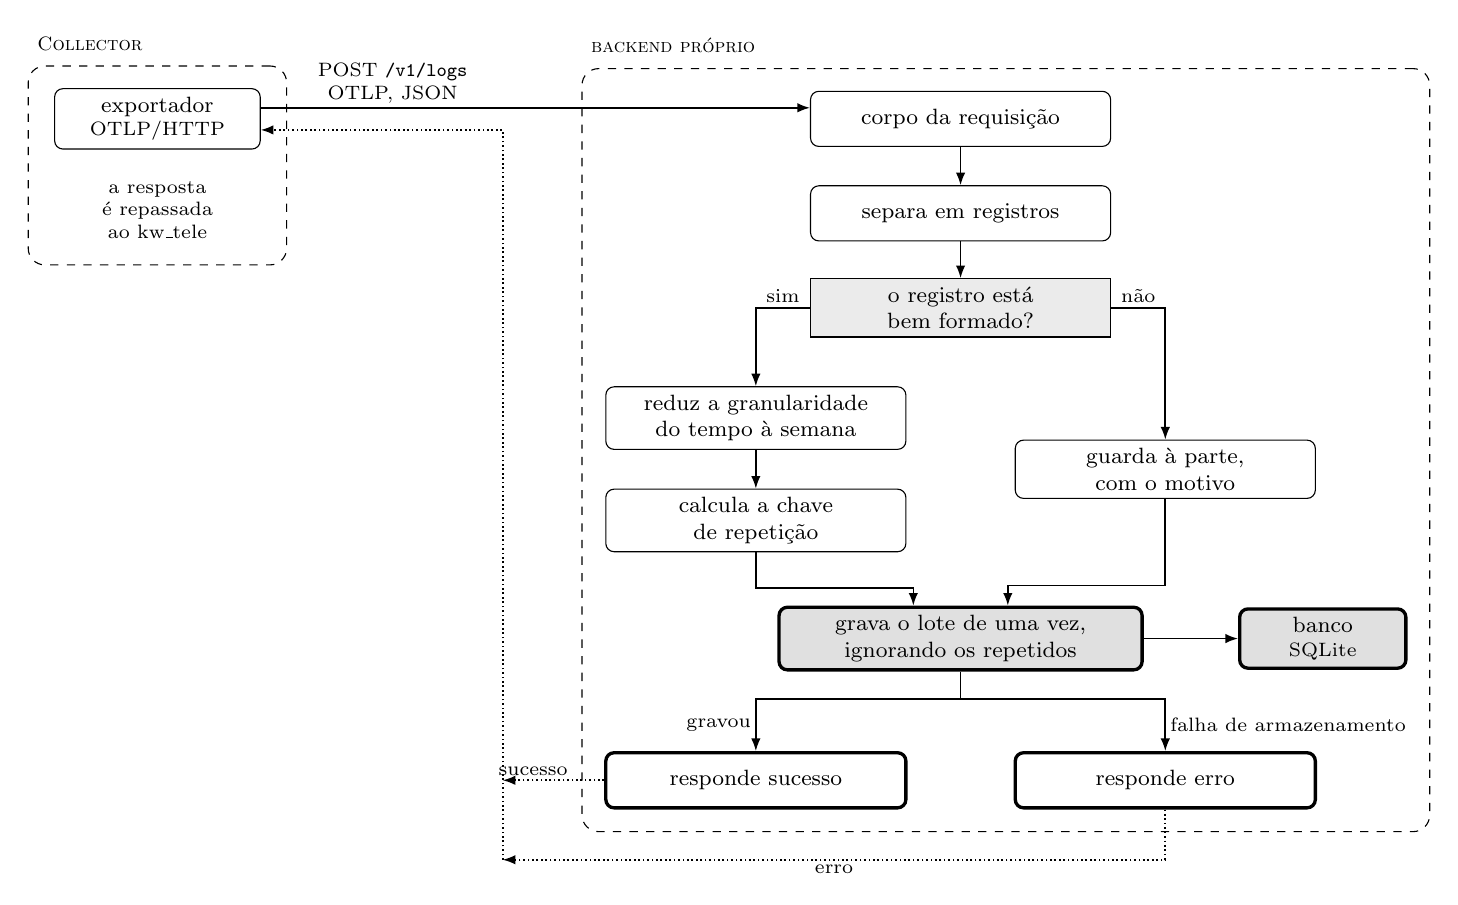
\begin{tikzpicture}[
    x=1cm, y=1cm,
    every node/.style={font=\footnotesize, align=center},
    passo/.style={draw, rounded corners=3pt, minimum height=0.7cm,
                  inner sep=3pt, fill=white, text width=3.6cm},
    pergunta/.style={draw, minimum height=0.7cm, inner sep=3pt,
                  fill=black!8, text width=3.6cm},
    dado/.style={passo, very thick, fill=black!12},
    fim/.style={passo, very thick},
    lado/.style={draw, dashed, rounded corners=6pt, inner sep=8pt},
    rotulo/.style={font=\scriptsize\scshape, anchor=south west},
    seta/.style={-{Latex[length=1.6mm]}, semithick},
    volta/.style={-{Latex[length=1.6mm]}, semithick, densely dotted},
    nota/.style={font=\scriptsize, inner sep=1.5pt},
  ]
  \node[passo] (corpo) at (0, 0) {corpo da requisição};
  \node[passo] (separa) at (0, -1.2) {separa em registros};
  \node[pergunta] (bom) at (0, -2.4) {o registro está bem formado?};
  \node[passo] (tempo) at (-2.6, -3.8) {reduz a granularidade do tempo à semana};
  \node[passo] (dup) at (-2.6, -5.1) {calcula a chave de repetição};
  \node[passo] (aparte) at (2.6, -4.45) {guarda à parte, com o motivo};
  \node[dado, text width=4.4cm] (grava) at (0, -6.6) {grava o lote de uma vez, ignorando os repetidos};
  \node[dado, text width=1.9cm] (sql) at (4.6, -6.6) {banco\\[-1pt]{\scriptsize SQLite}};
  \node[fim] (ok) at (-2.6, -8.4) {responde sucesso};
  \node[fim] (erro) at (2.6, -8.4) {responde erro};

  \node[lado, fit=(corpo)(tempo)(aparte)(sql)(ok)(erro)] (back) {};
  \node[rotulo] at ([yshift=2pt]back.north west) {backend próprio};

  \draw[seta] (corpo) -- (separa);
  \draw[seta] (separa) -- (bom);
  \draw[seta] (bom.west) -| node[nota, above, pos=0.25] {sim} (tempo.north);
  \draw[seta] (bom.east) -| node[nota, above, pos=0.25] {não} (aparte.north);
  \draw[seta] (tempo) -- (dup);
  \draw[seta] (dup.south) -- ++(0, -0.45) -| ([xshift=-0.6cm]grava.north);
  \draw[seta] (aparte.south) -- ++(0, -1.1) -| ([xshift=0.6cm]grava.north);
  \draw[seta] (grava) -- (sql);
  \draw[seta] (grava.south) -- ++(0, -0.35) -| node[nota, left, pos=0.75] {gravou} (ok.north);
  \draw[seta] (grava.south) -- ++(0, -0.35) -| node[nota, right, pos=0.75] {falha de armazenamento} (erro.north);

  \node[passo, text width=2.4cm] (exp) at (-10.2, 0) {exportador\\[-1pt]{\scriptsize OTLP/HTTP}};
  \node[nota, text width=2.6cm, anchor=north] (repassa) at ([yshift=-0.35cm]exp.south) {a resposta é repassada\\ao kw\_tele};
  \node[lado, fit=(exp)(repassa)] (col) {};
  \node[rotulo] at ([yshift=2pt]col.north west) {Collector};

  \draw[seta] ([yshift=4pt]exp.east) -- node[nota, above, pos=0.24, align=center] {POST \texttt{/v1/logs}\\OTLP, JSON} ([yshift=4pt]corpo.west);

  \coordinate (trilho) at ([xshift=-1.0cm]back.west);
  \draw[volta] (ok.west) -- node[nota, above, pos=0.7] {sucesso} (ok.west -| trilho);
  \draw[volta] (erro.south) -- ([yshift=-0.35cm]erro.south |- back.south) coordinate (e1) -- node[nota, below, pos=0.5] {erro} (e1 -| trilho);
  \draw[volta] (e1 -| trilho) |- ([yshift=-4pt]exp.east);
\end{tikzpicture}
}
  \caption{A entrada do backend próprio. A granularidade do tempo é reduzida à
    semana antes do cálculo da chave de repetição, e o lote é gravado de uma
    vez, sem os repetidos, antes da resposta.}
  \label{fig:backend-entrada}
\end{figure}

O backend próprio guarda os dados em três tabelas
(Figura~\ref{fig:esquema-backend}). Cada requisição recebida vira uma linha numa
tabela de lotes, com o momento da chegada, em granularidade de semana, e o
tamanho do corpo. Cada registro bem formado vira uma linha numa tabela de
registros, ligada ao seu lote: ela tem uma coluna para cada campo fixo do OTLP,
como a instalação, o corpo, o tempo do evento, o da observação e o
identificador do evento, e guarda todos os atributos juntos, num único
documento JSON. Os registros malformados vão para uma terceira tabela, também
ligada ao lote, com o motivo e o corpo como chegou. Não há uma coluna por
atributo nem uma tabela por fonte: um atributo novo é só mais uma chave no
documento, e a consulta o lê pelo nome (Seção~\ref{sec:extensibilidade}). O
preço é que o banco não sabe o tipo de cada atributo: a consulta agrupa pelos
valores lidos como texto e só soma uma medida onde o valor é numérico,
contando à parte os que não são.

\begin{figure}[!ht]
  \centering
  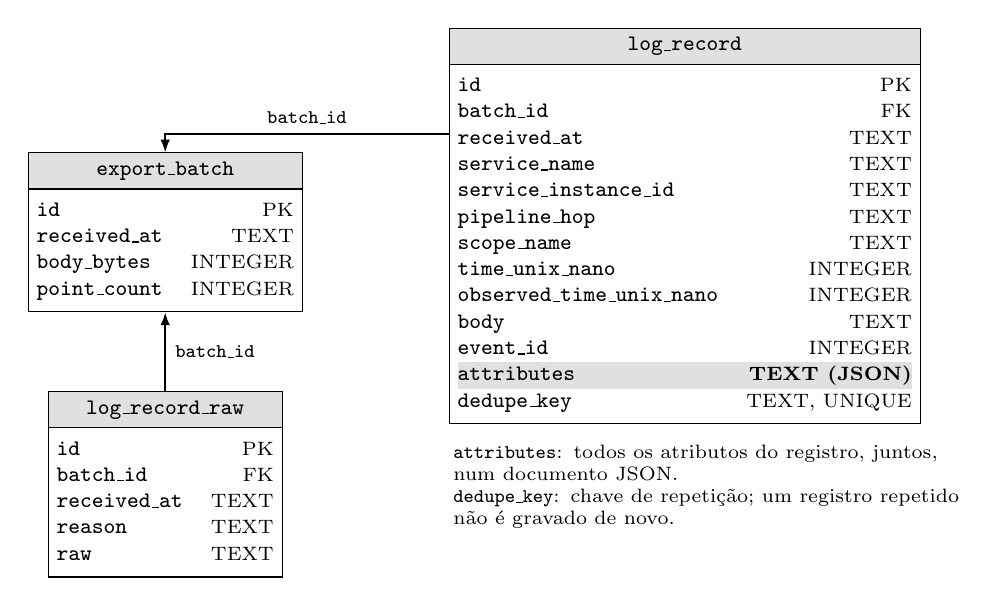
\begin{tikzpicture}[
    x=1cm, y=1cm,
    every node/.style={font=\footnotesize},
    tabela/.style={draw, rectangle split, rectangle split parts=2,
                   rectangle split part fill={black!12, white},
                   inner sep=3pt, font=\footnotesize},
    fk/.style={-{Latex[length=1.6mm]}, semithick},
    nota/.style={font=\scriptsize, align=left, inner sep=1.5pt},
  ]
  \providecommand{\kwcolunas}{}\renewcommand{\kwcolunas}[1]{%
    {\setlength{\tabcolsep}{0pt}\begin{tabular}{@{}l<{\hspace{1.2em}}@{}r@{}}#1\end{tabular}}}
  \providecommand{\kwcol}{}\renewcommand{\kwcol}[2]{\texttt{#1} & {\scriptsize #2}\\}
  \providecommand{\kwdestaque}{}\renewcommand{\kwdestaque}[2]{%
    \rowcolor{black!12}\texttt{\textbf{#1}} & {\scriptsize\textbf{#2}}\\}

  \node[tabela] (batch) at (0, 0) {%
    \texttt{export\_batch}
    \nodepart{two}
    \kwcolunas{\kwcol{id}{PK}\kwcol{received\_at}{TEXT}\kwcol{body\_bytes}{INTEGER}%
             \kwcol{point\_count}{INTEGER}}};

  \node[tabela, anchor=north west] (log) at (3.6, 2.6) {%
    \texttt{log\_record}
    \nodepart{two}
    \kwcolunas{\kwcol{id}{PK}\kwcol{batch\_id}{FK}\kwcol{received\_at}{TEXT}%
             \kwcol{service\_name}{TEXT}\kwcol{service\_instance\_id}{TEXT}%
             \kwcol{pipeline\_hop}{TEXT}\kwcol{scope\_name}{TEXT}%
             \kwcol{time\_unix\_nano}{INTEGER}\kwcol{observed\_time\_unix\_nano}{INTEGER}%
             \kwcol{body}{TEXT}\kwcol{event\_id}{INTEGER}%
             \kwdestaque{attributes}{TEXT (JSON)}%
             \kwcol{dedupe\_key}{TEXT, UNIQUE}}};

  \node[tabela] (raw) at (0, -3.2) {%
    \texttt{log\_record\_raw}
    \nodepart{two}
    \kwcolunas{\kwcol{id}{PK}\kwcol{batch\_id}{FK}\kwcol{received\_at}{TEXT}%
             \kwcol{reason}{TEXT}\kwcol{raw}{TEXT}}};

  \draw[fk] (log.west |- 0, 1.25) -| node[above, font=\scriptsize, pos=0.25] {\texttt{batch\_id}} (batch.north);
  \draw[fk] (raw.north) -- node[right, font=\scriptsize] {\texttt{batch\_id}} (batch.south);

  \node[nota, anchor=north west, text width=6.6cm] at ([yshift=-0.2cm]log.south west)
    {\texttt{attributes}: todos os atributos do registro, juntos, num
     documento JSON.\\
     \texttt{dedupe\_key}: chave de repetição; um registro repetido não é
     gravado de novo.};
\end{tikzpicture}

  \caption{O banco do backend próprio. Os atributos de cada registro ficam
    juntos num documento JSON; não há coluna por atributo nem tabela por
    fonte.}
  \label{fig:esquema-backend}
\end{figure}

Em seguida, o backend reduz de novo a granularidade do tempo à semana, para
que a regra valha também contra um cliente antigo ou de outra origem
(Seção~\ref{sec:mapeamento}); o Collector, como vem, não altera o tempo, e por
isso a regra fica no backend. É a única regra por campo aplicada no Collector
ou no backend. Com o tempo já reduzido, o backend calcula para cada registro
uma chave de repetição. Um registro com identificador de evento, como os que o
kw\_tele envia, é reconhecido pela instalação, pelo seu corpo e por esse
identificador; como o tempo deixou de distinguir um evento de outro, é o
identificador que faz esse papel.

Por fim, o backend grava o lote inteiro de uma vez, ignorando os registros
cuja chave já existe, e só então responde com sucesso; um reenvio, portanto,
não duplica nada. Se a gravação falha, ele responde com erro, e nada daquele
lote conta como recebido. Essa ordem é o que sustenta a cadeia de confirmação de ponta a ponta
(Figura~\ref{fig:confirmacao}). O kw\_tele só marca uma linha como enviada quando recebe uma
resposta de sucesso. O Collector só responde com sucesso depois que o backend
respondeu, porque não tem lote nem fila que o deixem responder antes. E o
backend só responde depois de gravar. Assim, um sucesso visto pelo kw\_tele
quer dizer que o lote foi gravado, com o que não coube no formato guardado à
parte.

Se o backend está parado, o Collector devolve erro, o kw\_tele não marca nada
e as linhas continuam pendentes; o próximo envio as manda de novo, e o
descarte de repetidos garante que um reenvio depois de uma falha parcial não
duplica registros. O padrão do exportador do Collector é ligar fila e novas
tentativas \citep{otel_collector_exporterhelper_v0_121_0}; elas foram
desligadas aqui para que a resposta de sucesso só venha depois da gravação.
Uma fila persistente no Collector, alternativa para uso em produção, não foi
construída.

\begin{figure}[!ht]
  \centering
  \resizebox{\textwidth}{!}{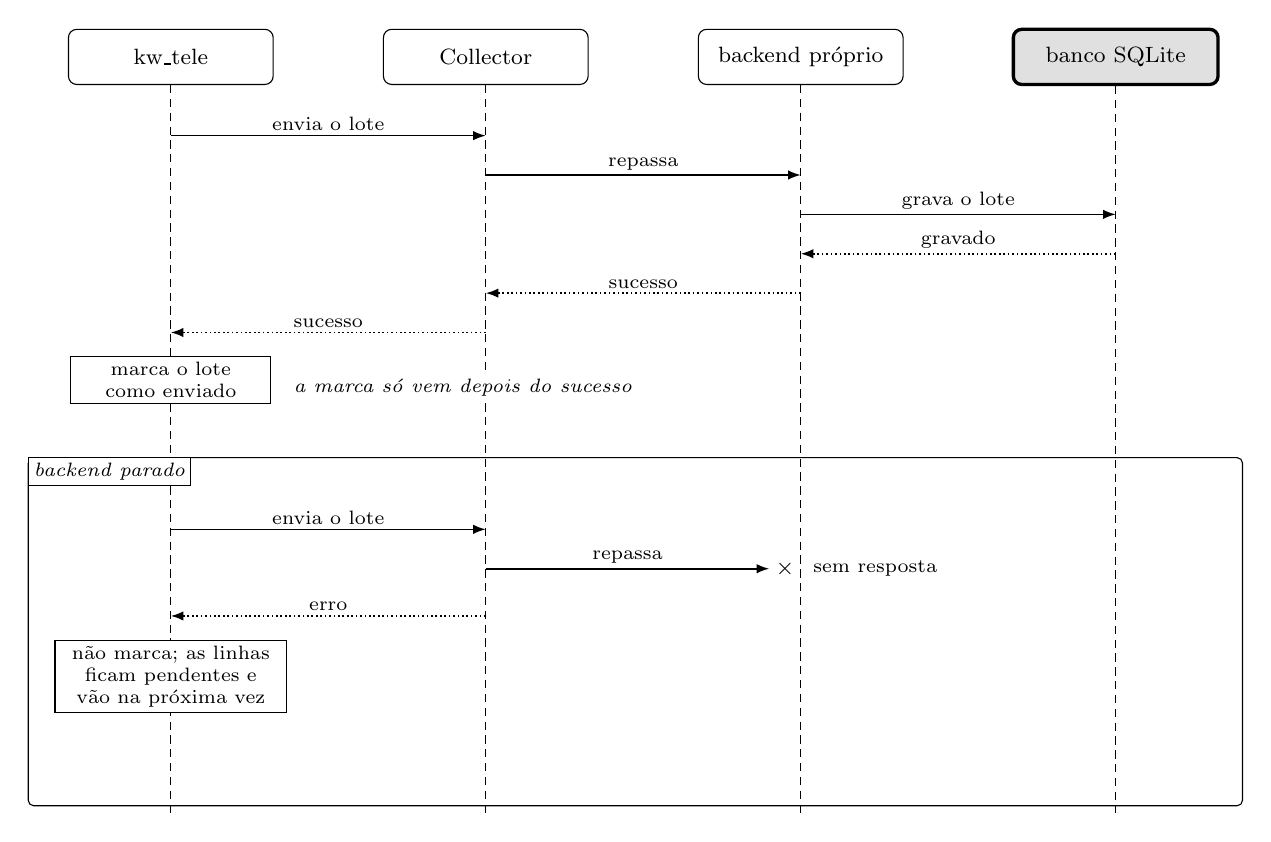
\begin{tikzpicture}[
    x=1cm, y=1cm,
    every node/.style={font=\footnotesize, align=center},
    ator/.style={draw, rounded corners=3pt, minimum height=0.7cm, minimum width=2.6cm,
                 inner sep=3pt, fill=white},
    dado/.style={ator, very thick, fill=black!12},
    vida/.style={densely dashed, thin},
    msg/.style={-{Latex[length=1.6mm]}, semithick},
    resp/.style={-{Latex[length=1.6mm]}, semithick, densely dotted},
    nota/.style={font=\scriptsize, inner sep=1.5pt},
    acao/.style={draw, fill=white, font=\scriptsize, inner sep=2pt, text width=2.4cm},
    quadro/.style={draw, rounded corners=2pt, inner sep=6pt},
    etiqueta/.style={draw, fill=white, font=\scriptsize\itshape, inner sep=2pt, anchor=north west},
  ]
  \foreach \n/\x/\t in {k/0/kw\_tele, c/4/Collector, b/8/backend próprio} {
    \node[ator] (\n) at (\x, 0) {\t};
    \draw[vida] (\n.south) -- (\x, -9.6);
  }
  \node[dado] (s) at (12, 0) {banco SQLite};
  \draw[vida] (s.south) -- (12, -9.6);

  \draw[msg] (0, -1.0) -- node[nota, above] {envia o lote} (4, -1.0);
  \draw[msg] (4, -1.5) -- node[nota, above] {repassa} (8, -1.5);
  \draw[msg] (8, -2.0) -- node[nota, above] {grava o lote} (12, -2.0);
  \draw[resp] (12, -2.5) -- node[nota, above] {gravado} (8, -2.5);
  \draw[resp] (8, -3.0) -- node[nota, above] {sucesso} (4, -3.0);
  \draw[resp] (4, -3.5) -- node[nota, above] {sucesso} (0, -3.5);
  \node[acao, anchor=north] at (0, -3.8) {marca o lote como enviado};

  \draw[msg] (0, -6.0) -- node[nota, above] {envia o lote} (4, -6.0);
  \draw[msg] (4, -6.5) -- node[nota, above] {repassa} (7.6, -6.5);
  \node[font=\footnotesize\bfseries] at (7.8, -6.5) {$\times$};
  \node[nota, right] at (8.1, -6.5) {sem resposta};
  \draw[resp] (4, -7.1) -- node[nota, above] {erro} (0, -7.1);
  \node[acao, anchor=north, text width=2.8cm] at (0, -7.4) {não marca; as linhas ficam pendentes e vão na próxima vez};
  \node[quadro, fit={(-1.6, -5.3) (13.4, -9.3)}] (alt) {};
  \node[etiqueta] at (alt.north west) {backend parado};

  \node[nota, anchor=west, font=\scriptsize\itshape, fill=white] at (1.5, -4.2) {a marca só vem depois do sucesso};
\end{tikzpicture}
}
  \caption{A confirmação. O kw\_tele só marca o lote como enviado depois que o
    sucesso volta do backend próprio, pelo Collector; com o backend parado, as
    linhas ficam pendentes.}
  \label{fig:confirmacao}
\end{figure}

\section{Consulta dos dados}
\label{sec:consulta}

O caminho descrito até aqui termina numa linha gravada pelo backend, e essas
linhas só servem se puderem ser lidas. O artigo do kw lista como alvos de
medição, por exemplo, em que hardware se compila e quem está sobrecarregado na
hierarquia de mantenedores (Seção~\ref{sec:dados-de-uso}); outros autores vão
querer outras coisas, e o backend não sabe de antemão que tipos de registro nem
que atributos vão chegar (Seção~\ref{sec:backend}). Por isso nenhuma consulta é
escrita para uma fonte: a pergunta chega como parâmetro. O backend próprio, o
mesmo que recebe os registros do Collector, oferece para isso três rotas, todas
só de leitura. Duas descrevem o que há nos dados, e a terceira agrupa e conta
(Figura~\ref{fig:consulta}).

\begin{figure}[!ht]
  \centering
  \resizebox{\textwidth}{!}{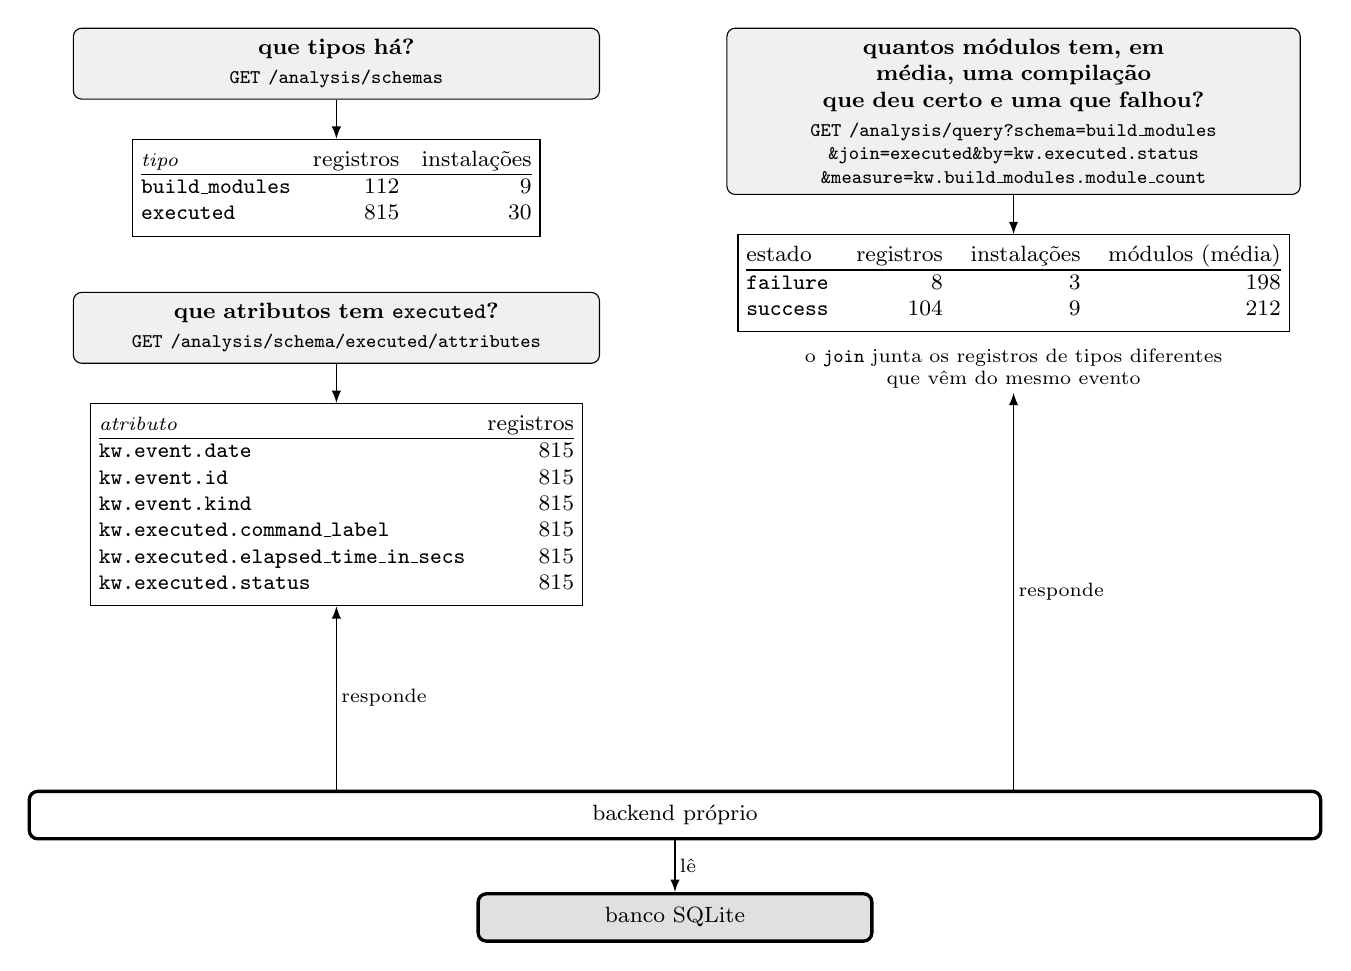
\begin{tikzpicture}[
    x=1cm, y=1cm,
    every node/.style={font=\footnotesize},
    pedido/.style={draw, rounded corners=3pt, inner sep=4pt, fill=black!6, align=center, text width=6.4cm},
    resp/.style={draw, inner sep=3pt, fill=white},
    dado/.style={draw, very thick, rounded corners=3pt, fill=black!12, inner sep=5pt, align=center},
    seta/.style={-{Latex[length=1.6mm]}, semithick},
    nota/.style={font=\scriptsize, align=center, inner sep=1.5pt},
  ]
  \node[pedido, anchor=north] (q1) at (0, 0) {\textbf{que tipos há?}\\[1pt]{\scriptsize\texttt{GET /analysis/schemas}}};
  \node[resp, anchor=north] (r1) at ([yshift=-0.5cm]q1.south) {%
    \setlength{\tabcolsep}{4pt}%
    \begin{tabular}{@{}lrr@{}}
      \scriptsize\textit{tipo} & registros & instalações \\
      \hline
      \texttt{build\_modules} & 112 & 9 \\
      \texttt{executed}       & 815 & 30 \\
    \end{tabular}};

  \node[pedido, anchor=north] (q2) at ([yshift=-0.7cm]r1.south) {\textbf{que atributos tem \texttt{executed}?}\\[1pt]
    {\scriptsize\texttt{GET /analysis/schema/executed/attributes}}};
  \node[resp, anchor=north] (r2) at ([yshift=-0.5cm]q2.south) {%
    \setlength{\tabcolsep}{4pt}%
    \begin{tabular}{@{}lr@{}}
      \scriptsize\textit{atributo} & registros \\
      \hline
      \texttt{kw.event.date}                       & 815 \\
      \texttt{kw.event.id}                         & 815 \\
      \texttt{kw.event.kind}                       & 815 \\
      \texttt{kw.executed.command\_label}          & 815 \\
      \texttt{kw.executed.elapsed\_time\_in\_secs} & 815 \\
      \texttt{kw.executed.status}                  & 815 \\
    \end{tabular}};

  \node[pedido, anchor=north, text width=7.0cm] (q3) at (8.6, 0) {\textbf{quantos módulos tem, em média, uma compilação}\\
    \textbf{que deu certo e uma que falhou?}\\[1pt]
    {\scriptsize\texttt{GET /analysis/query?schema=build\_modules}}\\[-1pt]
    {\scriptsize\texttt{\&join=executed\&by=kw.executed.status}}\\[-1pt]
    {\scriptsize\texttt{\&measure=kw.build\_modules.module\_count}}};
  \node[resp, anchor=north] (r3) at ([yshift=-0.5cm]q3.south) {%
    \setlength{\tabcolsep}{5pt}%
    \begin{tabular}{@{}lrrr@{}}
      estado & registros & instalações & módulos (média) \\
      \hline
      \texttt{failure} &   8 & 3 & 198 \\
      \texttt{success} & 104 & 9 & 212 \\
    \end{tabular}};
  \node[nota, anchor=north, text width=6.8cm] (j) at ([yshift=-0.15cm]r3.south)
    {o \texttt{join} junta os registros de tipos diferentes\\que vêm do mesmo evento};

  \node[draw, very thick, rounded corners=3pt, fill=white, inner sep=5pt, minimum width=16.4cm, align=center] (back) at (4.3, -10.0) {backend próprio};
  \node[dado, minimum width=5.0cm] (db) at (4.3, -11.3) {banco SQLite};
  \draw[seta] (db.north |- back.south) -- node[nota, right] {lê} (db.north);

  \draw[seta] (q1) -- (r1);
  \draw[seta] (q2) -- (r2);
  \draw[seta] (q3) -- (r3);
  \draw[seta] (back.north -| r2.south) -- node[nota, right] {responde} (r2.south);
  \draw[seta] (back.north -| r3.south) -- node[nota, right] {responde} (j.south -| r3.south);

\end{tikzpicture}
}
  \caption{As rotas de consulta sobre o banco do backend próprio. Valores
    ilustrativos.}
  \label{fig:consulta}
\end{figure}

A primeira rota devolve os tipos de registro que existem, isto é, os corpos,
que são os nomes das tabelas de extensão (Seção~\ref{sec:mapeamento}), cada
um com o número de registros e de instalações distintas. A segunda recebe um
desses tipos e devolve os atributos que aparecem nele, com quantos registros
têm cada um. É o ponto de partida quando não se sabe o que o kw grava: um tipo novo, como o da lista de módulos, aparece na primeira rota assim
que o primeiro registro dele é gravado, e os seus atributos, na segunda
(Seção~\ref{sec:extensibilidade}).

A terceira rota recebe um tipo e agrupa os seus registros pelos atributos
pedidos; se pedido, também resume uma medida numérica, como a duração de uma
execução. Os grupos podem ainda ser separados por semana, a granularidade com
que o tempo chega, e por instalação. A instalação aparece como um rótulo de ordem, e não com o seu identificador; o
risco desse rótulo está no Capítulo~\ref{cap:privacidade}. Antes
de agrupar, a consulta pode restringir os registros a um valor de atributo e a
um intervalo de semanas. Cada grupo traz o número de registros e o número de
instalações distintas. Os valores são agrupados como texto, e a medida só é
somada onde o valor é numérico, com os demais contados à parte, porque os atributos são guardados sem tipo.

Como cada fonte é um tipo separado, uma pergunta que cruza fontes precisa
juntar os registros. A terceira rota aceita outros tipos para juntar ao
pedido, ligando os registros do mesmo evento pela instalação e pelo identificador do
evento, que o cliente envia em todo registro e que o usuário não pode excluir
(Seção~\ref{sec:mapeamento}); um registro sem instalação ou sem esse
identificador não se junta a nenhum outro.
Com os dados de demonstração, a contagem de módulos vem dos registros da lista
de módulos e o estado da execução vem dos de execução. Juntando os dois tipos,
uma pergunta possível é se as compilações que falham têm mais módulos que as
bem-sucedidas; outra, sem junção, é quantas compilações terminaram em cada
estado a cada semana.

A consulta só devolve agregados: nenhuma rota devolve um registro individual
nem o identificador real de uma instalação, e os registros brutos ficam com
quem opera o backend. Ela também não traz painel nem gráfico. A resposta é um documento JSON, para
ser lida por um programa ou levada a uma ferramenta de análise, que também
poderia ler o mesmo banco SQLite; na leitura deste trabalho, é o mínimo para
responder a uma pergunta sem escrever código para ela. A falta de supressão de
grupos pequenos e de autenticação nas rotas são limites tratados no
Capítulo~\ref{cap:privacidade}, e a consulta sobre dados de várias
instalações é mostrada no Capítulo~\ref{cap:validacao}. A mesma consulta serve
a qualquer fonte que chegue pelo caminho (Seção~\ref{sec:extensibilidade}).

\section{Extensibilidade do sistema}
\label{sec:extensibilidade}

O sistema é extensível porque o conhecimento sobre o dado mora num ponto só, o
esquema do kw, e o resto do caminho o descobre em vez de o trazer escrito. A
Tabela~\ref{tab:extensao} resume o argumento, componente a componente, para uma
fonte nova. O kw é o único lugar que muda: a fonte nova é uma tabela ligada ao
evento e o código do kw que a preenche. O kw\_tele não precisa ser alterado,
porque descobre no esquema do banco as tabelas que estendem o evento e
transforma cada coluna num atributo (Seção~\ref{sec:mapeamento}). O protocolo
também não, porque ele define os atributos do registro de \textit{log} como
pares de chave e valor, sem fixar as chaves
\citep{otel_common_spec_v1_63_0,otlp_spec_1_11_1}, e um tipo novo é apenas
outro valor no corpo do registro. O Collector não olha os atributos. A exceção é o tempo: uma coluna de tempo própria da extensão sai como foi
gravada, porque a redução da granularidade só vale para as colunas do evento
(Seção~\ref{sec:mapeamento}).

\begin{table}[!ht]
  \centering
  \footnotesize
  \setlength{\tabcolsep}{4pt}
  \begin{threeparttable}
    \caption{O que muda em cada componente quando entra uma fonte nova, como a
      lista de módulos da compilação. Só o kw muda; a exceção é uma coluna de tempo na tabela nova, que não tem
      a granularidade reduzida no cliente.}
    \label{tab:extensao}
    \begin{tabular}{@{}>{\raggedright\arraybackslash}p{2.4cm}
                      >{\raggedright\arraybackslash}p{4.6cm}
                      >{\raggedright\arraybackslash}p{7.2cm}@{}}
      \toprule
      Componente & O que muda para uma fonte nova & Por quê \\
      \midrule
      kw & uma tabela cuja chave é o identificador do evento, e o código que a preenche
         & é onde o dado nasce \\
      \addlinespace[2pt]
      kw\_tele & nada
         & descobre no esquema as tabelas que estendem o evento \\
      \addlinespace[2pt]
      protocolo & nada
         & o registro de log carrega atributos livres, e o tipo é um valor do corpo \\
      \addlinespace[2pt]
      Collector & nada
         & não olha os atributos \\
      \addlinespace[2pt]
      backend próprio & nada
         & guarda os atributos juntos, sem uma coluna por atributo \\
      \addlinespace[2pt]
      consulta & nada
         & descobre nos dados os tipos e os atributos, e recebe o nome do
           atributo como parâmetro \\
      \bottomrule
    \end{tabular}
    \begin{tablenotes}
      \footnotesize
      \item Justificativas na Seção~\ref{sec:extensibilidade}.
    \end{tablenotes}
  \end{threeparttable}
\end{table}


No backend próprio, os atributos de cada registro são guardados juntos, num
documento JSON, e não numa coluna para cada um; a tabela de registros não
depende, assim, de que atributos chegam nem de como se chamam
(Figura~\ref{fig:esquema-backend}). A consulta descobre nos próprios dados os
tipos de registro e os atributos que existem, recebendo o nome do atributo como
parâmetro (Seção~\ref{sec:consulta}). Nenhum componente depois do kw conhece
fonte alguma, e por isso não há nada a registrar quando uma fonte aparece. A
privacidade acompanha o dado novo do mesmo modo: a exclusão de campos é uma
lista de chaves de atributo, e uma chave listada vale para o atributo que a
tiver, exista ele ou não no momento em que o usuário a configurou
(Capítulo~\ref{cap:privacidade}). Esse é o critério de extensibilidade da
Seção~\ref{sec:criterios} visto pelo lado do design, e é o que o sexto objetivo
deste trabalho pede (Seção~\ref{sec:objetivos}).

Um exemplo torna o argumento concreto: a lista de módulos de uma compilação,
isto é, os módulos que a configuração do kernel marca para serem compilados à
parte. Ela foi acrescentada ao kw como exemplo do argumento, e não por ser um
dado escolhido para coleta. No kw, e só nele, ela é uma tabela ligada ao evento da compilação ou da
instalação e o código que a preenche (Seção~\ref{sec:banco-local}). Uma
compilação ou uma instalação passa a gerar dois registros com o mesmo
identificador de evento, um por tabela, e a chave de repetidos do backend, que
inclui o corpo, os mantém separados. A prova de que o exemplo passa pelo
caminho, sem mudança no kw\_tele nem no backend, está no
Capítulo~\ref{cap:validacao}.

%!TeX root=../main.tex

\chapter{Implementação do protótipo}

\label{cap:implementacao}

O Capítulo~\ref{cap:solucao} disse o que cada componente faz e por quê; este
diz como cada um foi construído, para quem quiser ler o código ou reproduzir
o protótipo. O código está em dois repositórios: o \textit{fork} do kw, no
ramo de telemetria \citep{kwfork_telemetry}, e o repositório deste trabalho,
com o kw\_tele, a configuração do Collector, o backend próprio e a
demonstração \citep{tccrepo}. As mudanças no kw ficam nesse ramo e não foram
propostas ao projeto. O capítulo segue o caminho do dado, do kw ao backend, e
termina nos testes.

\section{As mudanças no kw}
\label{sec:impl-kw}

A telemetria entra no kw por um único ponto: o script principal carrega o
disparador antes de escolher o comando a rodar (Programa~\ref{prog:entrada}).
O arquivo é lido com o \texttt{.} do Bash, e não com a função
\texttt{include} do kw, porque a função cria um processo a mais e esse trecho
roda em todo comando. O ramo acrescenta ao kw cerca de 3,6 mil linhas em 30 arquivos,
das quais 2,7 mil são testes; do resto, a maior parte é o disparador, com
pouco mais de 400 linhas, e o comando \texttt{kw telemetry}, com pouco mais de
100 \citep{kwfork_telemetry}.

\begin{program}[htbp]
  \centering
\begin{lstlisting}[language=bash, style=wider]
# Plain `.` instead of `include`, which forks `realpath`: this runs on every
# command. A partial installation just skips the gate.
if [[ -r "${KW_LIB_DIR}/lib/telemetry.sh" ]]; then
  . "${KW_LIB_DIR}/lib/telemetry.sh" --source-only &&
    telemetry_gate "$action"
fi
\end{lstlisting}
  \caption{O ponto de entrada do disparador no script principal do kw, antes
    da escolha do comando; a última chamada foi quebrada em duas linhas para
    caber na página \citep{kwfork_telemetry}.}
  \label{prog:entrada}
\end{program}

No banco, o arquivo do esquema, \texttt{database/kwdb.sql}, ganhou a coluna de
marca de envio na tabela de eventos, a tabela da lista de módulos e uma
\textit{view} de inserção com um gatilho que grava o evento, a execução e os
módulos numa instrução só. É o gatilho que torna a escrita atômica: uma
segunda chamada ao \texttt{sqlite3} não saberia o identificador do evento que
a primeira acabou de criar. A gravação dos módulos é chamada pelo
\texttt{build.sh} e pelo \texttt{deploy.sh}, com sucesso ou falha. A
verificação do esquema, para os bancos já instalados, acrescenta a coluna e um
índice dos eventos pendentes e reaplica o arquivo do esquema se a \textit{view} da lista de módulos faltar. Por fim, os comandos do kw passaram a esperar até 5 segundos quando o
banco está ocupado, para que a escrita do kw não falhe enquanto o kw\_tele
marca linhas.

O disparador segue a ordem da Figura~\ref{fig:disparador}. Ele lê a configuração e o estado com o próprio Bash e, no caminho comum, só
consulta o banco para contar os eventos pendentes; a verificação do esquema
roda apenas antes de perguntar o consentimento ou de disparar o kw\_tele. Para
disparar, ele usa \texttt{setsid}, que separa o kw\_tele do terminal, e
\texttt{timeout}, que limita a sua duração. Ele nunca
escreve na saída do comando nem muda o código de saída dele; a pergunta de
consentimento vai para a saída de erro.

O comando \texttt{kw telemetry} reúne o
que o usuário faz com a telemetria: ver o que foi gravado e enviado, enviar
ou ver o próximo lote sem enviar, aceitar ou recusar, e mudar a configuração;
o ramo acrescenta a página de manual correspondente. A configuração,
\texttt{etc/telemetry.config}, tem as chaves do comportamento descrito na
Seção~\ref{sec:cliente}: o intervalo entre envios, o tempo mínimo entre
tentativas, o tamanho do lote, o endereço e a lista de exclusão, que vem vazia. O
consentimento fica preso ao endereço aceito: se o endereço muda à mão, o kw
pergunta de novo.

O \texttt{setup.sh} do kw instala o kw\_tele. O caminho previsto é baixar a
versão publicada no repositório deste trabalho; enquanto não há versão
publicada, o kw\_tele é construído a partir de uma cópia local do repositório,
indicada por uma variável de ambiente. Numa reinstalação, o kw\_tele antigo é mantido até o novo ser instalado. Se a instalação falha, o \texttt{setup.sh}
avisa e continua, e o kw funciona sem telemetria, porque o disparador vê que o
kw\_tele não está instalado. A única dependência nova declarada para as
distribuições é o Python.

%!TeX root=../main.tex

\chapter{Validação do protótipo}

\label{cap:validacao}

%!TeX root=../main.tex

\chapter{Privacidade, consentimento e anonimização}

\label{cap:privacidade}

\section{O que a telemetria do kworkflow exporia}

\section{Modelo de consentimento}

\section{Anonimização e riscos residuais de reidentificação}

%!TeX root=../main.tex

\chapter{Conclusão}

\label{cap:conclusao}


%%%%%%%%%%%%%%%%%%%%%%%%%%%%%%%%% REFERÊNCIAS %%%%%%%%%%%%%%%%%%%%%%%%%%%%%%%%%%%

\backmatter

\pagestyle{backmatter}

\printbibliography[
  title=\refname\label{sec:bib},
  heading=bibintoc,
]

\end{document}
